\documentclass[11pt]{article}
%Gummi|063|=)
\usepackage{amsmath}
\usepackage[utf8]{inputenc}
\usepackage[authoryear, round]{natbib}
\usepackage{graphicx}
\usepackage[inner=2.5cm,outer=2.5cm,bottom=2cm]{geometry}
\usepackage{mathrsfs}
\usepackage{subfig}


\title{\textbf{Predicting Economic Time-Series using Dynamic Factor Models under Structural Breaks}}
\author{Johannes Degn}
\date{07.07.2014}
\begin{document}


\maketitle
\thispagestyle{empty}
\setcounter{page}{0}

\newpage
\tableofcontents
\newpage
\listoffigures
\listoftables
\newpage




\section{Introduction}
Factor models are used in a wide range of situations spanning from economic indices over prediction of high-dimensional datasets. The basic idea is that there are unobservable factors driving the change of the variables of interest. Put differently, it is assumed that the change of variables is composed of a common component affecting all variables in the set and an idiosyncratic component which is specific to the variable of interest.

If the common factors can be derrived consistently they can prove to be a valuable and possibly less noisy set of predictors for the variables of interest than the whole set of available variables. Nowadays, typically the factors are estimated using principal components analysis. Resultingly factor models harbor similarity to principal component regression including the feature of dimensionality reduction which allows both models to be estimated even if the number of columns exceeds the number of rows. This is precisely what makes factor models appealing in a macroeconomic forecasting context. There exist many international macroeconomic variables some of which are not covered over a very long time horizon. With factor models all this information can be used directly.

In a time-series framework an interesting question to ask is whether these common components are stable over time or if the relationship of the variables of interest with the underlying factors are prone to changes. While there are recent additions to the field, the behaviour of factor models under structural breaks is still being researched. There are at least two reasons why structural breaks are interesting in an econometric model. If we assume that strcutural breaks imply a change in the coefficients of the model at a certain period, this can be interesting in itself especially if the coefficients and the factors are to be interpreted directly. Additionally, from a forecasting perspective it can be worthwhile to consider only the data after the structural break(s) has happened\footnote{Alternatively, instead of splitting the data into multiple periods for each break, a single forecasting equation can be constructed which includes the structural break by introducing a dummy variable.}. The hope is that the parameters of the model which are estimated relying only on the data after the last break might be closer to the true values which have generated the data to be forecast. This assumes that there will not be another structural break at the period which is be forecast. It should be notet that \citet{pesaran2007selection} have shown that it can be slightly better to include same observations before the last break.

This thesis deals with testing for structural breaks in factor models and using factor models for forecasting in a situation where structural breaks might be present.\footnote{Structural breaks can refer to changes in the means and variances of variables or a change in the relationship of variables. I focus on the latter. More specificity will be added in section 3.} \\
The contribution is twofold: Firstly, the influence of structural breaks on factor models is examined. To this end feasible testing procedures developed by \citet{breitung2011testing} are presented. Bootstrap versions of these chow type tests are developed and their performance is evaluated. Secondly, the information about the structural breaks is used for forecating. The performance of different model specifications is tested in the form of horse races. The competing models are:
\begin{enumerate}
	\item A static factor model with no structural breaks (but with more factors)
	\item A static factor model with structural break(s)
	\item A dynamic factor model with no structural breaks
	\item A dynamic factor model with structural break(s)
\end{enumerate}

The paper is structured into X parts. Firstly factor models are introduced. Both static and dynamic models are presented along with some theory and estimation methods. Secondly structural breaks are introduced, their effects on the factors and loadings are looked at and testing methods are considered. Thirdly aforementioned models are estimated using both syntetic and real data. Finally the fourth part concludes. \\

Throughout this thesis I will assume that $X$ is a matrix of potentially very many predictors. To stay consistent with existing literature I will index $X$ with $i$ or $t$ interchangeably where $i$ stands for the column index and $t$ for the row index. Also as is customary, throughout this paper capital letters denote matrices while lower case letters denote vectors except for innovation terms which are always in lower case letters. All variables containing data are assumed to be demeaned and normalized to have unit variance\footnote{I.e. every variable $y_t$ is derrived as $y_t = \frac{y_t^* - \bar y_t}{\sigma_{y}}$ where $y_t^*$ is the vector containing the original data and $\sigma_{y}$ is the (sample) standard deviation of $y$}.

\section{Factor Models}
As mentioned, the idea behind factor models or diffusion index models is that there are underlying latent factors which explain the evolution of the observable variables $X$. 

They are ususally written in the form of a factor equation (\ref{factor equation}) and a forecasting equation (\ref{forecasting equation}). 
\begin{equation}
	\label{factor equation}
	X_t = \lambda(L) f_t + e_t
\end{equation}
\begin{equation}
	\label{forecasting equation}
	y^h_{t+h} = \alpha(L) W_t + \beta(L) \hat f_t + \varepsilon_{t+h}
\end{equation}
	
$X_t$ is a $N \times 1$ vector of potentially very many predictors. $\lambda(L)$ is a $N \times q$ matrix of lag polynomials, $f_t$ is a $q \times 1$ vector of latent factors. $e_t$ is a $N \times 1$ vector of idiosyncratic errors which may or may not be serially auto-correlated. $W_t$ consists of variables which the researcher knows to be sufficiently relevant to enter the forecasting equation directly. Usually $W_t$ is taken to consist of s lags of $y_t$ and a constant term. $\hat f_t$ is an estimate of the factors in the factor equation (\ref{factor equation}). Estimation of the factors is treated below.

Most authors assume the idiosyncratic component to be a white noise process (i.e. independent and of mean 0), however "weak" dependence is also commonly assumed. In the vocabulary of factor models these are models with uncorrelated idiosyncratic components $e_t$ (more specifically $E(e_t e_t') = \Sigma = \text{diag}(\sigma_{e_1}^2, ..., \sigma_{e_N}^2)$ and $E(e_t) = 0$).

\citet{geweke1977dynamic} and \citet{sargent1977business} distinguish between exact or strict Factor Models and approximate Factor Models. In essence the difference is composed of different assumptions for the error terms. Approximated factor models allow for limited correlatedness of the idiosyncratic innovations $e_{it}$ between periods while strict factor models do not. More precise deifinitions follow now and are taken from \citet{breitung2006dynamic}
\subsubsection*{Strict factor models}
\citet{breitung2006dynamic} list the assumptions for strict factor models as follows: For the innovations it is assumed $E(e_t) = 0$ and $E(e_te_t') = \sigma = \text{diag}(\sigma_1^2, ..., \sigma_N^2)$. Also $E(f_t) = 0$ and $E(f_tf_t') = \Omega$. If $E(f_t) = 0$ it follows that $E(X_t) = 0$ which is enforced by demeaning the variables. Additionally $E(f_t e_t') = 0$ i.e. the innovations and the error terms are uncorrelated. It follows directly that $E(X_tX_t') = \Lambda \Omega \Lambda' + \Sigma$\footnote{$E(X_tX_t') = E[(\Lambda f_t +e_t) (\Lambda f_t + e_t)'] = E(\Lambda f_t f_t' \Lambda' + \Lambda f_t e_t' + e_t f_t' \Lambda' + e_t e_t') = \Lambda \Omega \Lambda' + \Sigma$}
\subsubsection*{Approximate factor models}econo
Approximate factor models losen the assumptions of strict factor models at the cost of assuming $N \to \infty$.
$E(e_{it}e_{js})$ is allowed to be different from $0$ but only weakly. Similarly the factors $f_t$ and and the idiosyncratic error terms are allowed to be correlated but again only weakly, so that $E(f_t e_t')$ does not have to be $0$. But $N^{-1}\Lambda'\Lambda$ must converge to a positive definite limiting matrix $\Sigma_\Lambda$ which ensures that the factors influence each variable with a similar order of magnitude. Otherwise it could be that the loadings for some variables are $0$ \citep{breitung2006dynamic}. Similiary it is assumed about the factors that $T^{-1}\sum_{t=1}TF_tF_t' \overset{p}{\to} \Sigma_F$. This allows for stationary processes e.g. an ARMA process. \\
Some more assumptions are necessary for the inferential theory\footnote{Most notably the results of \citet{bai2003inferential} are consistency and normality of the factor estimations. The rate of convergence is shown to be $\min(\sqrt{N}, \sqrt{T})$.} of \citet{bai2003inferential} to hold. Namely these assumptions are Assumptions A through D in \citet{bai2003inferential}:

\begin{flalign*}
	\textbf{Assumption A: } E||F_t||^4 \leq M < \infty \text{ and } T^{-1} \sum_{t=1}^TF_t F_t' \overset{p}{\to} \Sigma_F \text{ for some } r \times r \text{ positive matrix } \Sigma_F &\\
\end{flalign*}

\begin{flalign*}
	\textbf{Assumption B: } ||\lambda_1|| \leq \bar \lambda < \infty, \text{ and } || \Lambda' \Lambda/N - \Sigma_\Lambda|| \to 0 \text{ for some } r\times r \text{ positive definite matrix } \Sigma_\Lambda & \\
\end{flalign*}

\begin{flalign*}
	&\textbf{Assumption C: } \exists M: 0<M < \infty \text{ such that } \forall N, T, &\\
	&\text{1.) } E(e_{it}) = 0, E|e_{it}|^8 \leq M &\\
	&\text{2.) } E(e_s'e_t/N) = E(N^{-1} \sum_{i=1}^N e_{is} e_{it}) = \gamma_N(s, t), |\gamma_N(s, s)| \leq M \forall s \text{ and } &\\
	&T^{-1}\sum_{s=1}^T \sum_{t=1}^T | \gamma_N(s, t) \leq M &\\
	& \text{3.) } E(e_{it}'e_{jt}) = \tau_{ij, t} \text{ with } |\tau_{ij, t}| \leq |\tau_{ij}| \text{ for some } \tau_{ij} \text{ and for all } t \text{ and } &\\
	& N^{-1} \sum_{i=1}^N \sum_{j=1}^N |\tau_{ij} \leq M &\\
	& \text{4.) } E(e_{it}'e_{js}) = \tau_{ij, ts} \text{ and } (NT)^{-1} \sum_{i=1}^N\sum_{j=1}^N\sum_{t=1}^T\sum_{s=1}^T|\tau_{ij, ts}| \leq M &\\
	& \forall (t,s) E\left| N^{-1/2} \sum_{i=1}^N[e_{is}e_{it} - E(e_{is}e_{it})]\right|^4 \leq M &\\
\end{flalign*}

\begin{flalign*}
	&\textbf{Assumption D: } E(\frac{1}{N} \sum_{i=1}^N || \frac{1}{\sqrt{N}}\sum_{t=1}^TF_t e_{it} || ^2) \leq M &\\
\end{flalign*}

Assumption C allows for some degree of dependence and heteroskedasticity among the innovation terms which will be used below to simplify the calculation of the dynamic factor model. \\


As mentioned, an important advantage of factor models compared to simpler econometric models is that they do not necessarily suffer if the fraction $\frac{T}{N}$ becomes small whereas most models can not cope with more variables than observations. VAR models for example have the problem that the number of parameters to estimate becomes too high quickly if $N$ is high relative to $T$. 
The reason why factor models do not have this problem is that firstly the factor equation is estimated. This gives estimates $\hat f_t$ of the factors. Then only the first $r$ eigenvectors are used in the forecasting equation where $r<N$\footnote{Typically $r$ is much smaller than $N$. E.g. the famous one factor model of intelligence by \citet{spearman1904general} (in which factor models were developed the first time) has $r=1$.}. This feature allows researchers in principle to append $X$ by further variables derived from the initial set. \citet{bai2008forecasting} for example use what they call squared principal components and quadratic principal components. The first of which appends squares of the $X_i$ to the initial matrix $X$ such that $X_{t}^{spc}=\left\{X_{it}, X_{it}^2\right\}$ and the second of which adds the cross products of $X_i$ such that $X_t^{qpc} = \left\{ X_{it}, X_{it} X_{jt}\right\} \forall i \not= j$. The idea is to change the link function between $X_t$ and $f_t$ from being linear to allow for a nonlinear relationship. \citet{bai2008forecasting} also consider adding a squared term of the factors $f_t$ to the forecasting equation (\ref{forecasting equation}) to allow the volatility of the factors to influence the forecast. Naturally, the value of these approaches depends heavily on what is being forecasted. \\

Apart from the distinction into strict or approximate factor models, a further distinction can be made between static and dynamic factor models. This distinction concerns the relationship between lags of $f_t$ and $X$. Static models set $\alpha(L)$ to be of lag order $0$ while dynamic models alow for dependence with other lag orders.


\subsection{Static Factor Models}
For static factor models $X_t$ depends only on $f_t$ and not on lags of $f_t$ i.e. factors enter only contemporaneously. Resultingly a static factor model is the case in which the lag order in equation (\ref{factor equation}) is 0.


\begin{equation}
	\label{factor equation, t indexed}
	X_t = \Lambda F_t + \bar e_t
\end{equation}

Where $X$ is a $T \times N$ Matrix of predictors. $F$ is a $T \times r$ factor matrix. $\Lambda$ is a $N \times r$ loadings matrix. $\bar e$ is a $T \times N$ matrix of idiosyncratic errors. $C$ is called the common component.
Note that depending on whether authors index by row, column or both, several alternative ways of writing down the factor model equation are used in the literature.

\begin{equation}
	\label{factor equation, it indexed}
	X_{it} = \Lambda_i' F_t + \bar e_{it}
\end{equation}
\begin{equation}
	\label{static factor equation}
	X = F \Lambda' + e = C + \bar e
\end{equation}
\begin{equation}
	\label{factor equation, i indexed}
	X_i = F_i \lambda + \bar e_i
\end{equation}





\subsection{Dynamic Factor Models}
In applications there will usually be some kind of time dependence structure. Thus, dynamic factor models introduce a dynamic process into the factors.

\begin{equation}
	\label{time dependence of factors}
	f_t = \Psi(L) f_{t-1} + \eta_t \text{\ \ \ \ \ (VAR representation)}
\end{equation}

In practice it is usually easier to ignore the dynamic process in the factors $f_t$ and follow e.g. \citet{stock2005implications} among others in assuming a dynamic proccess in the innovation term of the factor equation (\ref{factor equation}) instead. This captures the dynamic process while avoiding the technical difficulty in estimating the dynamic factors themselves. The underlying thought is that there will be some residual autocorrelation if the dynamic process of the factors is not modelled explicitely which can be caught by an AR(p) process for the innovation term \citep{breitung2011gls}. Additionally the lag polynomial $\lambda(L)$ in the factor equation (\ref{factor equation}) captures the noncontemporaneous interactions of the factors $f_t$ and $X_t$.

For the purpose of this paper I assume the following AR processes for the innovation term of the dynamic factor models \citep{breitung2011testing}.
\begin{equation}
	\label{AR process innovation term}
	e_{it} = \varrho_{i,1} e_{i, t-1} + ... + \varrho_{i, p_i} e_{i, t-p_i} + \xi_{it} \text{ where $\xi_{it}$ is white noise}
\end{equation}


\subsubsection{Static interpretation of dynamic factor models}
Dynamic factor models can be written as static factor models in a linear state space environment. This gives the static factor equation (\ref{factor equation, t indexed}) and $\Phi(L) F_t = G \eta_t$ where $\Phi(L)$ is defined such that equivalence to (\ref{time dependence of factors}) holds and $F_t$ is defined below as the stacked lagged dynamic factors $f_t$ (\citet{stock2011dynamic}). \\

Solving the lag operator, we can write equation (\ref{factor equation}) in the form 
\begin{equation}
	\label{factor equation, solved lag polynomial}
	X_{it} = \lambda_{i1}' f_t + ... + \lambda_{im}' f_{t-m} + e_{it}
\end{equation}
Following \citet{bai2002determining} this can be rewritten as 
$$X_{it} = \Lambda_i^{*'} F_t + e_{it}$$
$$\text{where } \Lambda_i^* = \begin{bmatrix} \lambda_{i1} \\ \lambda_{i2} \\ \vdots \\ \lambda_{im} \end{bmatrix} \text{ and } F_t = \begin{bmatrix} f_t \\ f_{t-1} \\ \vdots \\ f_{t-m} \end{bmatrix}$$

To keep consistency between variable naming schemes denote the dimension of $F_t$ as $r \times 1$ and the dimension of $\Lambda_i^*$ as $N \times r$. Thus we can always rewrite a dynamic factor model in static form and resultingly we can use the procedure introduced below to estimate the $r$ "static factors"\footnote{\citet{breitung2004identification} call the $f_t$ "structural factors" and the $F_t$ "reduced form" factors.} $F_t$ as specified below.
It can be seen that the dimension of the resulting stacked vector of "static" factors is $q(m+1)$ thus we can set $r=q(m+1)$. This shows that there is a relationship between $r$ and $q$ if the dynamic factor model is written as a static factor model. To identify $q$ it remains to estimate $m$.

There exist several ways to identify the dynamic factors from there\footnote{Note that identifying the dynamic factors might not be of interest for forecasting but rather that it is a necessary condition in order to interpret the factors in a dynamic factor model. For forecasting purposes, in order to choose the number of factors and the number of the factor lags used in the forecasting equation (\ref{forecasting equation}) one can also follow \citet{bai2008forecasting} in using the BIC criterion to choose both simultaneously. }. Firstly \citet{giannone2002tracking} suggest estimating the VAR $F_t = C F_{t-1} + \kappa_t$ and then to apply principal component analysis on an estimate of the residual covariance matrix (see \citet{breitung2004identification} or \citet{giannone2002tracking} for details). \citet{breitung2004identification} exploit the relationship between $q$ and $r$ in order to find information criteria which can determine $q$ and the lag order of the $\lambda$. This paper does not estimate the dynamic factors directly as in the application the factors are primarily used for the second stage regression. \\

Imagine the true data would be generated by a dynamic factor model. If instead of using the dynamic factor model specification and finding the dynamic factors from the static factors, a researcher simply estimates a static factor model it can be seen above that the number of factors $r$ will be larger than the number of dynamic factors $q$.

\subsection{Estimation of the factors}
\subsubsection{Static factors}
There exist now a number of ways to estimate the static factors $F$ in (\ref{static factor equation}). Ultimately what we are looking for is a solution to the minimization of the squared error.
\begin{equation}
	\label{factor equation minimization problem}
	\min_{F_1, ..., F_T, \Lambda} \frac{1}{NT} \sum_{t=1}^T (X_t - \Lambda F_t)'(X_t - \Lambda F_t)
\end{equation}

Since both $\Lambda$ and $F_t$ are unspecified, there are infinitely many solutions to (\ref{factor equation minimization problem}) and the problem is not identified. To achieve identification assumptions can most conveniently be put on either $\Lambda$ or $F_t$\footnote{\citet{bai2013principal} consider several alternative normalizations. They also show that direct interpretation of the factors and loading matrices are possible if one is willing to additionally assume diagonality of $\Lambda'\Lambda$ or that $\Lambda$ is a block matrix of 2 submatrices with one submatrix being triangular.}. Usually $\Lambda$ is normalized such that $N^{-1} \Lambda'\Lambda = I_r$. Alternatively $T^{-1}F'F = I_r$ is also frequently used. The choice of normalization can have a noticeable impact on the computational demand of calculating a solution for the minimization problem in (\ref{factor equation minimization problem}). The columns spaces spanned by the estimates of $F$ are equivalent with both normalizations \citep{stock2011dynamic}.

\citet{stock2011dynamic} list four ways which are being applied in the literature to get a solution $\hat F$ and $\hat \Lambda$ to the minimization problem (\ref{factor equation minimization problem}). Firstly a Gaussian process can be assumed which allows for maximum likelihood estimation using the Kalman filter. To do this a dynamic factor can be rewritten as a static factor model in a linear state space writing as mentioned above. \\
Secondly principal components (and other nonparametric averaging methods) can be used to estimate both $\hat F$ and $\hat \Lambda$ at the same time. This requires relatively weak assumptions and is particularly easy to and computationally efficient which explains both the popularity of this approach and why this approach is applied in this thesis. Additionally the principal component estimation can be generalized by weighting the minimization problem with the variance matrix of the error term to take account of error variances which are not prooportional to the identity matrix (see \citet{stock2011dynamic} for details). Evidence of performance improvements by using the generalized principal components approach over the standard principal components estimator are mixed. Resultingly the simpler principal components estimator will be used. It will be described in more detail below. An unattractive feature of principal component estimation is thaint it can not identify the "true" factors $f_t$ but rather a transformation $Q f_t$ for some undefined rotation matrix $Q$ which results in some difficulty in interpreting the factors directly. \citet{bai2013principal} show a minimum set of assumptions which are required in order to make valid interpretations of the estimated factor and loading matrices.

Principal Components estimation of the factors is asymptotically equivalent to maximum likelihood estimation if normality is assumed \citep{bai2003inferential}. \\
Thirdly mixture approaches between the two methods from above can be constructed. \\
Fourthly and finally Bayesian methods can be used to get estimations of the factors and loadings which can have computational advantages over the maximum likelihood approach and can be useful if the assumption of Gaussian error terms is unappealing. \\

The principal component method estimates $\hat F$ and $\hat \Lambda$ as follows. Normalizing $F$ such that $T^{-1}F'F = I_r$ gives $\hat F = \sqrt{T} * eigenvectors_r(XX')$ where $eigenvectors_i(A)$ returns the i eigenvectors corresponding to the i largest eigenvalues of a square matrix $A$. Since $\hat X = \hat F' \hat \Lambda$, it follows directly that we can estimate $\Lambda$ by $\hat \Lambda' = (\hat F' \hat F)^{-1} \hat F'X$. due to the normalization $\hat F' \hat F = T$ and we can write $\hat \Lambda = X' \hat F / T$. \\
If, alternatively, we apply the normalization $N^{-1}\Lambda'\Lambda = I_r$ the solution to (\ref{factor equation minimization problem}) becomes $\hat \Lambda = \sqrt{N} * eigenvectors_r(X'X)$. This solution to the optimization problem is shown in appendix \ref{Estimation of the Factor Equation}). Then we can follow from $\hat X = \hat F \hat \Lambda'$ that $\hat F = X \hat \Lambda (\hat \Lambda' \hat \Lambda)^{-1}$. Again due to the normalization $\Lambda' \Lambda = N$ and we can write $\hat F = X \hat \Lambda / N$.

Note that the normalization $T^{-1}F'F = I_r$ requires us to calculate the eigenvectors of $XX'$ which has dimension $T \times T$ while the alternative $N^{-1}\Lambda'\Lambda = I_r$ requires us to calculate the eigenvectors of $X'X$ which is $N \times N$. Depending on the relative sizes of $T$ and $N$ it can make a considerable difference in terms of computational burden which method is applied. \\

\textbf{The number of factors}
One important issue that remains to be addressed is the question of how many factors should be used in the factor equation. There exist many different ways that this choice can be made. Firstly there are simple rules of thumb. E.g. some researchers only consider factors with eigenvalues greater than $1$. Then there are methods which rely on a similar idea but employ graphical methods. The idea is to inspect the resulting scree plots\footnote{Scree plots plot the ordered eigenvalues against the number of factors (i.e. eigenvalues and corresponding eigenvectors) which results in a falling curve.}. The intuition is to only take factors into account if the eigenvalue corresponding to the next factor is smaller by a sufficient amount. This idea is also behind the cut-off value of 1 for eigenvalues. Basing on this, formal tests have been derrived which rely on the eigenvalues calculated above \citep{stock2011dynamic}.

The information criteria developed by \citet{bai2002determining} are perhaps more appealing as they formalize the costs and benefits of an additional factor explicitly \citep{stock2011dynamic}. \citet{bai2002determining} consider $6$ criteria, the first three of which they call $PCp$ criteria (Panel $C_p$ criteria). These criteria result from a generalization of Mallows' $C_p$ \citep{mallows1973some}. The second set of $3$ criteria refine the usual criteria used in time-series analysis to depend on both $N$ and $T$. \citet{bai2002determining} highlight that the criteria $IC_{p1}$, $IC_{p2}$, $PC_{p1}$ and $PC_{p2}$ are specifically suited for principal component estimation. \citet{bai2002determining} present a montecarlo study to highlight the differences between the criteria. Notably the $PC_{p}$ criteria require the specification of a maximum number of factors, the choice of which is quite arbitrary\footnote{In their montecarlo study \citet{bai2002determining} set the maximum number of factors to be $8$ noting that they used the rule in \citet{schwert2002tests} and that one could consider $kmax=\text{int}[(\min\left\{N, T\right\}/100)^{1/4}]$. Tests which are not presented here show that choosing a different $kmax$ can result in the $PC_p$ criteria to become quite unstable. Especially high values of $kmax$ often result in the maximum number of factors chosen such that $r=kmax$}. Resultingly this paper uses the $IC_p$ criteria. Specifically the $IC_{p2}$ criterion because it seems to be more conservative (i.e. it usually underestimates $r$ whereas $IC_{p2}$ overestimates at times). 

In order to understand the criteria better, tables 1 and 2 of \citet{bai2002determining} have been replicated using both different values for $r$ and $kmax$. If $r$ is chosen as in \citet{bai2002determining}, the replicated results are almost identical to the original calculations and thus are not reported\footnote{I.e. differences are so small that they can be explained by sampling variation.}. The results can be found in two tables in appendix \ref{bai ng information criteria}. Tables I through VIII in \citet{bai2002determining} in essence show $3$ points. Firstly, traditional criteria perform poorly in estimating the number of factors if compared to the $6$ presented criteria. Of the newly developed information criteria $PC_{p1}$, $PC_{p2}$, $IC_{p1}$ and $IC_{p2}$ perform well even under heteroskedasticity and autocorrelation. Secondly, if $\min\{N, T\}$ becomes too small, the performance of the criteria suffers which is highlighted by the bottom 5 results in the tables. Especially $PC_{p3}$ suffers in this regard. In the given specifications the cut-off value for $\min\{N, T\}$ appears to be 40 or 60 if the variance of the innovations is high. Thirdly, $PC_{p3}$ and $IC_{p3}$ are less robust to a small $\min\{N, T\}$. \\
The replication results in appendix \citet{bai2002determining} harbor three additional insights. Firstly as $r$ increases, the requirements for $\min\{N, T\}$ are also higher. For $r=7$ and $r=9$ it seems $\min\{N, T\}$ should be at least $100$. Secondly the choice of $kmax$ can matter a lot. Especially for small samples the specification of $kmax=8$ used in \citet{bai2002determining} choose the maximum number of factors frequently when the $N$ and $T$ are too small. Almost all results in the last 5 rows set $\hat k=8$ whereas the replicated results often report a lower number of factors if $kmax=\text{ceil}(\min\{T, N\})$. Noticeably, this also happens in the replicated results for $r \in \{1, 3, 5\}$ and $kmax=\text{ceil}(\min\{T, N\})$. If $kmax=\text{ceil}(\min\{T, N\})$ $IC_{p3}$ predicts $\hat k=50$ in the $T=100, N=100$ case for $r \in \{1, 3, 5, 7, 9\}$. Thus, the choice of $kmax$ can have a huge impact on the prediction of the number of factors. Luckily it is typically easy to see when the information criteria choose all the factors. In those cases the plausibily of the results should be checked by hand. \\

An interesting question if one is ultimately interested in forecasting is whether the "true" number of factors is of any interest at all or if the number of factors used in the forecasting equation (\ref{forecasting equation}) should perhaps be different from the predicted $r$ in the static model or $q$ in the dynamic model. The answer can not be easily given. Similar to \citet{bai2008forecasting} we can dodge this question somewhat by using the BIC criterion to choose a model among a list of models with differing number of factors (or number of lags of the variable of interest).

\citet{breitung2011testing} among others, however, note that if one is primarily interested in forecasting, the number of dynamic factors can be ignored and a static factor model with a higher number of factors can be estimated with equivalent success.


\subsection{Forecasting}
The forecasting equation (\ref{forecasting equation}) can be estimated using a simple linear regression of $y_{t+h}$ on $\hat F_t$, $y_t$, lags of $y_t$ and depending on the model specification lags of $\hat F_t$.

The performance of factor models for forecasting purposes is most pronounced if the number of variables used in the factor equation is high \citep{stock2011dynamic}. This makes sense because more variables improve the fit of the factor equation. However, there is a trade-off between quantity and quality of variables\footnote{I.e. a smaller set of variables with a high predictive power can outperform a larger set of variables which includes the variables from the smaller set} that should not be ignored. This case will be adressed in the next subsection.

\subsubsection{Targeted predictors}
\citet{bai2008forecasting} follow the idea that if factor models are ultimately going to be used for forecasting it might make sense to "target" the set of predictors $X_t$ to the task of forecasting the variable of interest $y_t$. The idea stems from \citet{boivin2006more} who find that selecting only the "informative" variables can yield better results than taking a bigger set of variable which include the same "informative" variables but also additional ones. \citet{bai2008forecasting} thus provides a formal rule for which variables should be used for forecasting. To that end they use hard and soft thresholding rules to preselect among the predictors $X_t$ those that have a meassurable influence on $y_t$. Resultingly, a subset $\tilde X_t \subset X_t$ is selected for estimating the factor equation, the hope being that then the factors are better suited for predicting $y_t$.

 For hard thresholding they regress $y_t^h$ on $W_{t-h}$ and $X_{it-h}$ for each $i=1, ..., N$\footnote{Note that the $N$ regressions include only the lags and single predictors $X_i$ as independent variables.}. Then they compare the resulting t-statistics to a threshold and discard those predictors whose t-statistics do not exceed that threshold. For soft thresholding \citet{bai2008forecasting} perform penalized regressions, LASSO, elastic net and Least Angle Regression (see \citet{tibshirani1996}, \citet{zou_hastie2005}, \citet{efron_hastie_johnstone_tibshirani2004} for details) using the fact that these regression specifications set the parameters of variables which are not important to $0$. \\

It should be noted that this approach, while attractive in principle, requires additional thought in the presence of structural breaks.


\subsection{Interpreting the factors}
TODO: should I include such a chapter? It would involve finding out which variables the factors load onto.

\subsection{Applications}
Factor models have been applied in a wide range of different domains apart from economics. Most notably psychology and biology. Staying in the realms of economics, prominently, there are applications in the calculation of indices. The is based on the idea that the factors consist of underlying tendencies applying to all variables which makes them appealing as tools to generate indices.

\citet{schumacher2010factor} employs a similar idea in that he uses international predictors to forecast German GDP. Firstly it is intuitive that international data has an influence on an open economy directly. But secondly it is conceivable that there are underlying factors which influence both German GDP growth and international macroeconomic variables at the same time. However, to make sure that the information conveyed in the additional international predictors is of relevance for forecasting, \citet{schumacher2010factor} "targets" the predictors prior to esimating the factor equation, as described above.


TODO: see Bai (2003) page 1 for more examples!

\section{Structural breaks}
The treatment of structural breaks follows \citet{breitung2011testing} closely. The question of interest is how a researcher should react to structural breaks in the factor equation.

The factor model under a structural breaks in period $T^*$ can be written as follows:
\begin{equation}
	\label{}
	y_{it} = f'_t\lambda_i^{(1)} + \varepsilon_{it} \text{ for } t = 1, ..., T^*
\end{equation}
\begin{equation}
	\label{}
	y_{it} = f'_t\lambda_i^{(2)} + \varepsilon_{it} \text{ for } t = T^* + 1, ..., T
\end{equation}

The intuition is the same as with simpler models: a structural break implies a different relationship between the variable of interest and the factors and hence different factor loadings for the periods before and after the breaks. Multiple structural breaks can be specified accordingly. In theory, structural breaks could be also thought of as affecting the forecasting equation (\ref{forecasting equation}). This is ignored here because structural breaks in equations of this type have been thoroughly researched.


Interestingly, estimating a static factor model without structural breaks if the true data generating process includes structural breaks, yields an analogy to ignoring dynamic factors if they were present in the data generating process: the space estimated by the factors will be of higher dimension. This means that the number of factors $r$ predicted e.g. by the \citet{bai2002determining} information criteria will be higher than if no structural breaks were present. \citet{breitung2011testing} note that similar to dynamic factor models it is enough to increase the number of factors if one is primarily interested in decomposing the common component from the idiosyncratic component (that is to say if one is interested foremost in forecasting).

If structural breaks are detected in one or more of the factors the question remains what should be done next. Since structural breaks consist of an instability in the factor loadings at a certain period it can be optimal in a forecasting sense to estimate the respective parameter after the structural break has occured in the hope that this new parameter value contains more accurate information about the future. There is of course a trade-off here because the data series is shorter afterwards which has a negative effect on prediction accuracy.
An alternative approach consists of removing the variable containing the structural break from the data set. This approach allows all other series to enter the forecasting equation at the same length as before while the added noise through the structural breaks is removed. The idea is similar to targeted predictors which remove uninformative predictors from the data set in order to improve the ratio of information to noise. Because of the typically high dimension of the data matrix $X$, factor models appear to be well suited for the second approach. Which method should be chosen depends on the size of the structural break, the relative position of the break and the relative information content of the other variables. In practice it is necessary to test in order to weigh the benefits and costs. This is done in the empirical section.

\subsection{Testing for structural breaks}
\citet{breitung2011testing} develop several Chow type tests for the static factor model under the assumptions of the strict factor model. They also develop Quandt-Andrews type supremum tests. The test statistics are as follows.


\begin{equation}
	\label{LR-Statistic}
	\text{lr}_i = T [ \log(S_{0i}) - \log(S_{1i + S_{2i}}) ]
\end{equation}

Where $$S_{0i} = \sum_{t=1}^{T}(y_{it} - \hat{f_t'} \hat \lambda_i)^2 \text{, } S_{1i} = \sum_{t=1}^{T_1^*}(y_{it} - \hat{f_t'} \hat \lambda_i^{(1)})^2 \text{ and } S_{2i} = \sum_{t=T^*_i+1}^{T_1^*}(y_{it} - \hat{f_t'} \hat \lambda_i^{(2)})^2 $$
denote the residual sum of squares for the whole date range, the first subperiod up until the structural break and the period from the break to the end of the sample respectively.
$\hat \lambda^{(1)}$ and $\hat \lambda^{(2)}$ denote the esimated factor loadings calculated on the data before the break and after the break respectively.

\begin{equation}
	\label{LM-Statistic}
	\text{lm}_i = T R^2_i \text{ where $R_i^2$ is the r-squared from a regression } \hat \varepsilon_{it} = \theta_i' \hat f_t + \phi \hat f_t^* + \tilde \varepsilon_{it}
\end{equation}

\begin{equation}
	\label{Wald-Statistic}
	\text{wald}_i = \text{ Wald statistic for $H_0: \Psi_i = 0$ in the regression } y_{it} = \lambda_i' \hat f_t + \psi \hat f_t^* + \nu_{it}
\end{equation}

Where 
$$\hat f_t^* = \begin{cases} 0 \text{ for } t=1, ..., T_i^* \\ \hat f_t \text{ for } t=T_i^*+1, ..., T \end{cases}$$

\begin{equation}
	\label{LM-Statistic}
	\text{LM}^* = \frac{\left( \sum_{i=1}^N s_i \right) -rN}{\sqrt{2rN}}
\end{equation}

The LM$^*$ statistic pertains to the joint test of no structural break in all the factor loadings. Note, however, that the assumptions required for the LM$^*$ statistic are those of a strict factor model, namely no interdependence in the error terms $e_t$ in (\ref{factor equation}).

The LR, LM and Wald statistics defined above can be used to define a test for a unknown break date as in \citet{andrews1993tests}. Under mild assumptions \citet{breitung2011testing} show that the supremum statistic defined over the LM statistics is distributed using the nonstandard distribution given in \citet{andrews1993tests} and tabulated again in \citet{andrews2003tests}.

\begin{equation}
\label{sup LM statistic}
\mathscr{S}_{i,T}(\tau_0) = \sup_{\tau \in [\tau_0, 1-\tau_0]} (s_i^\tau) \text{ where $s_i^\tau$ refers to either the LR, LM or Wald statistic}
\end{equation}



As mentioned in the introduction of the dynamic factor model, I follow \citet{breitung2011testing} in assuming an AR(p) process for the innovation term as in equation (\ref{errors AR(p)}):
\begin{equation}
	\label{errors AR(p)}
	e_{it} = \varrho_{i, 1} e_{i, t-1} + ... + \varrho_{i, p_i} e_{i, t-p_i} + \xi_{it}
\end{equation}
This is in line with the assumptions of the approximate factor model introduced above.

For dynamic factor models\footnote{Note that \citet{breitung2011testing} call a model where the innovations are generated by an AR(p) model a dynamic model whereas the literature usually refers to a dynamic process in the factors as in equation (\ref{time dependence of factors}). This is similar in effect but not quite the same.} \citet{breitung2011testing} propose to use a GLS transformed model, i.e. to perform the regression:
$$\varrho_i(L) y_{it} = \lambda_i'[\varrho(L) \hat f_t] + \psi' [\varrho_i(L) \hat f_t^*] + \varepsilon^*_{it}$$
The lag polynomials are obtained by applying some information criterion to the $N$ regressions
$$\hat \varepsilon_{it} = \varrho_{i, t-1} \hat u_{i, t-1} + ... + \varrho_{i, p_i} \hat u_{i, t-p_i} + \tilde \varepsilon_{i,t}$$

Similar test statistics as above can then be applied to the results of the GLS regressions. \citet{breitung2011testing} only present the LM-statistic.
$$\hat \varrho_i(L) y_{it} = \lambda_i' \left[\varrho_i(L) \hat f_t\right] + \psi_i' \left[\hat \varrho_i(L) \hat f_t^*\right] + \tilde \varepsilon^*_{it} \text{ for } t= p_i+1, ..., T_i$$

Under heteroskedasticity the regression has to be weighted by the covariance matrix. If we also take account of the possibility of a break in the covariance matrix we get two distinct regressions
$$\frac{1}{\hat \sigma^{(1)}} \varrho_i(L) y_{it} = \lambda_i' \left[\frac{1}{\hat \sigma_i^{(1)}} \varrho_i(L) \hat f_t\right] + \left[\frac{1}{\hat \sigma_i^{(1)}} \varrho_i(L) \hat f_t^*\right] + \tilde \varepsilon^*_{it} \text{ for } t = p_i+1, ..., T^*_i$$
$$\frac{1}{\hat \sigma^{(2)}} \varrho_i(L) y_{it} = \lambda_i' \left[\frac{1}{\hat \sigma_i^{(2)}} \varrho_i(L) \hat f_t\right] + \left[\frac{1}{\hat \sigma_i^{(2)}} \varrho_i(L) \hat f_t^*\right] + \tilde \varepsilon^*_{it} \text{ for } t = T_i*+1, ..., T$$



\subsection{Bootstrapping \citet{breitung2011testing}}
In order to test whether the properties of the above test statistics can be improved upon I have repeated the montecarlo study presented in \citet{breitung2011testing} tables 2 and 3 with the difference that the test statistics have been bootstrapped. \\

The idea behind bootstrapping test statistics comes from the definition of the p-value. Denoting with $\tau$ the test statistic of interest, by $\hat \tau$ the realization of that test statistic given the observed data and by $F$ the cumulative distribution function $\tau$ under the null hypothesis we can borrow the notation from \citet{davidson2004econometric} and write the p-value as
$$p(\hat \tau) = 1 - F(\hat \tau)$$
Resultingly the p-value can be estimated by estimating $F(\hat \tau)$. To do this we will simulate new data which follows the DGP under $H_0$. The p-value is then the (estimated) probability of the test statistic exceeding the calculated value $\hat \tau$ if the hypothesis $H_0$ were true. \\

Again following \citet{davidson2004econometric} we denote with stars, values that are calculated from simulated data, $B$ denotes the number of simulated samples. We can then estimate the cumulative distribution function as 
$$\hat F^*(x) = \frac{1}{B} \sum_{j=1}^B I(\tau^*_j \leq x) \text{ and } \hat F^*(\hat \tau) = \frac{1}{B} \sum_{j=1}^B I(\tau^*_j \leq \hat \tau)$$
Resultingly
$$\hat p^*(\hat \tau) = 1 - \hat \hat F^*(\hat \tau) = 1 - \frac{1}{B} \sum_{j=1}^B I (\tau^*_j \leq \hat \tau) = \frac{1}{B}\sum_{j=1}^B I(\tau^*_j > \hat \tau)$$

In the following two specifications of the bootstrap are considered. Firstly, the often used resampling of the residuals is applied. Secondly the wild bootstrap is used. 

Resampling the residuals uses the definition of the factor equation (\ref{factor equation}) to generate new data. The innovation term $e_t$ is replaced with resampled residuals\footnote{Resampling is done with replacement to model the empirical distribution. So the resampled residuals $e_t^*$ are given by setting $\hat e_t^* = \hat e_s$ where $s$ is drawn from $\{1, ..., T\}$ with replacement.} gotten from the estimation of the model using the initial data.

\begin{equation}
	\label{factor equation, bootstrapped}
	X_t^* = \hat f_t \hat \Lambda' + \hat e_t^*
\end{equation}

The wild bootstrap serves to deal with heteroskedasticity. The idea is to rescale the residuals using a white noise random variable $\nu_t$.

$$X_t^* = \hat f_t \hat \Lambda' + \hat e_t^+$$
Where $\hat e_t^+$ is set such that to $\hat e_{it}^+ = \hat e_{it} \nu_{it}$ and $\nu_{it}$ is distributed with mean $0$ and variance $1$. For the application I choose $\nu$ to be standard normal.




\section{Notes on the Literature}
\citet{cragg1997inferring} shows in a Monte Carlo analysis that $T\rightarrow\infty$ and $N\rightarrow\infty$ makes that classical theory for predicting the number of factors performs badly. Resultingly information criteria as in \citet{bai2002determining} should be used. These results hold under heteroskedasticity and weak serial correlation. But: structural breaks! TODO!!




\section{Empirical application}
In this section I will approach the issue of forecasting economic time series in the presence of structural breaks. Specifically, I will focus on forecasting German GDP using German und US American macroeconomic time-series. The reason for including American time-series to predict German GDP is twofold. Firstly, Germany is active on international markets with the US being the second most important export market after France. Coupled with the big importance of the US American market in the world economy it is plausible that US data plays a role in predicting German economic development. Secondly, we are interested in forecasting time-series under structural breaks. There are at least two periods commonly associated with breaks in the world economy: the dot-com bubble of 2000 and the financial crisis of 2008, both of which originated in the US. The hope is that big ruptures in the world economy make a break of relationships between variables (and ultimately of the factor loadings) likely.

There are several ways to address the issue of structural breaks from a forecasting viewpoint. Firstly structural breaks can be ignored. As has been stated above, in this case factor models will tend to choose the a higher number of factors than if no structural breaks are present which is means that the space the factors span is of a higher dimension as the factors are orthogonal.\footnote{How this affects the information criteria of \citet{bai2002determining} can be seen in table 1 of \citet{breitung2011testing}.}

Secondly, structural breaks can be included in the model in the form of a dummy parameter interacting with the factor estimations $\hat f_t$. The forecasting equation of the model then results as
\begin{equation}
	\label{forecasting, structural breaks}
	y^h_{t+h} = \alpha(L) W_t + \beta(L) \hat f_t + \gamma(L) \hat f_t^* + \varepsilon_{t+h}
\end{equation}
where $\hat f_t^*$ is defined as above.

Thirdly, if predictors are to be targeted prior to estimating the factor equation it is conceivable to find that a subset of the predictors $\tilde X_t^{(1)} \subset X_t$ peforms well before and a different subset $\tilde X_t^{(2)} \subset X_t$ performs better after the structural break. This finding would imply that it could be beneficial to estimate the factor equation again using only the data after $T^*$ and discarding the rest.


\subsection{Data choice and treatment}
The data used for the horse race has been collected from the German Bundesbank and the the American Federal Reserve Bank of St. Louis.\footnote{More specifically the FRED2 public API has been used to extract selected series. The data from the Bundesbank have been scraped from the Bundesbank website.}  It consists of $T=82$ observations from $N=169$ quarterly variables. The series are listed below in appendix \ref{Data series}. The series contain macroeconomic variables such as wages and salaries, employment levels and survey data from Germany and the US as well as financial variables.

Additionally an emphasis has been put on selecting several time-series which are well known to be subjected to big changes in the abovementioned periods such as "Housing starts".


They have been downloaded in seasonally adjusted form where appropriate. The data series have then been differenced (zero times, once or twice) until stationarity. To this end the number of differencing operations necessary to make the series stationary have been tested using the KPSS method developed in \citet{kwiatkowski1992testing}.\footnote{The method consists of constructing an LM-test for the hypothesis that the variance $\sigma^2_\varepsilon$ is 0 (or equivalently that $\mu_t$ is constant) in $$y_t = \beta'D_t + \mu_t + u_t$$ $$\mu_t = \mu_{t-1} + \varepsilon_t$$ where $\varepsilon_t \sim N(0, \sigma^2_\varepsilon)$ and $D_t$ captures deterministic components and time trends. This implies that the difference of $y_t$ denoted $\Delta y_t$ is stationary.}

The series have been demeaned and normalized such that $\frac{1}{T}\sum_{t=1}^T X_{it} = 0 \ \forall i$ and $\frac{1}{T}\sum_{t=1}^T X_{it}^2 = 1 \Leftrightarrow \sum_{t=1}^T X_{it}^2 = T \ \forall i$. \\


\subsection{Model selection and evaluation}
This section explores the different methods to selected and evaluate a model. The ultimate goal is always forecasting the true data as closely as possible. To this end I use the root mean squared forecasting error (RMSE) as an evaluation mechanism. $RMSE = \sqrt{\frac{1}{w}\sum_{s=t}^{t+h}[(y_s - \hat y_s)^2]}$ where $w$ denotes the length of the window to be forecasted and $t$ the period preceding the window being forecasted. The estimates $\hat y_t$ are gotten from estimating the forecasting equation and predicting $h$ steps into the future.

If the number of static factors in the forecasting equation is predetermined using criteria defined above, the number of lags of the variable of interest $y_t$ and the number of lags of the static factors are still open. In the following I refer to the number of lags of $y_t$ as $s$. 

I follow \citet{bai2008forecasting} in selecting among model candidates using the BIC and the FPE criterion which are of course in-sample criteria. 

\citet{bai2008forecasting} write the BIC and FPE criteria as follows

\begin{equation}
\label{information criteria}
\begin{split}
	& \text{BIC} = \log(\hat \sigma_n^2) + n \frac{\log T}{T} \\ 
	& \text{FPE} = \log(\hat \sigma_n^2) + n \frac{2}{T}
\end{split}
\end{equation}

Where $\hat \sigma_n^2$ is the residual variance $\hat e'e$ from an estimation of the factor equation using $n$ predictors.

Since the point of the exercise is forecasting, additionally, the best model in terms of out-of-sample forecasting performance is calculated. This is done by calculating the root mean squared error of one step ahead pseudo out-of-sample forecasts.\footnote{Pseudo out-of-sample forecasts are a method to simulated a forecasting situation in that the forecaster does as if he would not know the true realizations of the data after $t$. The forecaster tries to predict the value $y_{t+h}$ given all the information up to $t$. $t$ is then successively moved one period ahead. Here we set $h=1$.} This evaluation method follows \citet{forni2005the} and \citet{bai2008forecasting} among others. The foreacasting window $w$ over which the pseudo out-of-sample-forecasts are performed is set to $w=15$ here. \\


All models are compared to a benchmark model which consists of a simple moving average over the forecasting window $w$. This forecasting window makes sure that there are more observations than parameters for all possible models. Since the length of the data series is $T=82$ this leaves $67$ observations for the first forecast in the pseudo out-of-sample procedure. The maximum number of factors is set to $15$ for static models and $10$ for dynamic models. The maximum number of lags of $y_t$ is set to $10$. This brings the maximal number of parameters to $n_{max} = 25$ for static models and $n_{max} = 50$ for dynamic models. The original number of predictors is $N = 169$ which highlights that factor models are are an appropriate way to deal with the situation of $N>>T$ in this data set.

The first panel in table \ref{results static factor model} shows the results of the in sample selection procedure for a static factor model. Three variants for choosing the number of factors are considered. Firstly the IC$_{p2}$ criterion from \citet{bai2002determining} is used to estimate the number of static factors for both the factor equation and the forecasting equation. The information criteria (BIC and FPE) are then used to select $s$, the number of lags of $y_t$.
As a second choice, the decision over the number of factors \textit{and} the number of lags of $y_t$ in the forecasting equation are left to the information criteria. I.e. the information criteria are minimized over different choices of $r$ and $s$. The same number of factors is used in the factor equation.
A third possibility consists of leaving the choice of the number of factors for the factor equation to a \citet{bai2002determining} criterion and using the BIC or FPE criterion to choose the number of static factors in the forecasting equation along with the number of lags of $y_t$. I.e. the BIC or FPE are minimized over $r$ and $s$.

Both the BIC and FPE as well as the $IC_{p2}$ criteria select a large number of factors. The fact that conventional information criteria should not be used for selecting the number of static factors has been extensively documented in the factor model literature and is no surprise. Another approach to model selection for forecasting consists of testing the model in an out-of-sample forecasting situation and selecting the best performing model in terms of the forecasting error. The results of optimal forecasting model are reported in the second panel of table \ref{results static factor model}.

Since the variance of the data series has been normalized to $1$ and the mean to $0$ the RMSE of the simple average $y_t$ in the given window can be expected to be close to $1$. The RMSE of the resulting out-of-sample forecasts is very large with $1.30$ and $1.22$ respectively. The benchmark model of a moving average reports an RMSE of $0.86$ and an AR(6) model achieves an RMSE of $0.50$ for the same time horizon.\footnote{$6$ is the optimal lag number in terms of RMSE.}

The best performing static factor model in terms of forecasting can be got if the BIC criterion for model selecting is replaced by the RMSE as can be seen in the second panel. I.e. the RMSE is minimized over choices of $r$ and $s$ rather than the BIC. This implies using the out-of-sample performance as an evaluation criterion. In that case both $r$ and $s$ are shrunken to $1$. While this outperforms the simple benchmark model, the fact that the most parsimonious static factor model performs best in out-of-sample prediction hints at possible performance increases if dynamic effects are allowed.

\begin{table}[ht]
\centering
\caption{Static factor model, model selection}
\label{results static factor model}
\begin{tabular}{c|llll}
  & $r_{factor}$ & $r_{forecast}$ & $s$ & RMSE\\
  \hline
  \hline
    & \multicolumn{3}{l}{\textit{In-Sample}} \\
	BIC & 13 & 13 & 5 & 1.30 \\
	FPE & 15 & 15 & 5 & 1.23 \\
	$IC_{p2}$ \& BIC & 4 & 13 & 5 & 1.30 \\
	$IC_{p2}$ \& FPE & 4 & 15 & 5 & 1.23 \\
	$IC_{p2}$ & 4 & 4 & 10 & 1.21 \\
  \hline
  \hline
  & \multicolumn{3}{c}{\textit{Out-of-Sample}} \\ 
   	RMSE & 1 & 1 & 1 & 0.71 \\
   	RMSE \& $IC_{p2}$ & 4 & 1 & 1 & 0.71 \\
  \hline
  \multicolumn{5}{l} {\rule{0pt}{2cm} \begin{minipage}{8cm}
		\small{\textbf{\textit{Notes:}} The results are derrived by minimizing the information criteria in the first column. If both an \citet{bai2002determining} criterion and a standard information criterion is given the former is applied to the factor equation and the latter to the forecasting equation. The maximum number of factors $r$ is set to $15$. The maximum number number of the lags of the variable of interest $s$ is set to $10$.}
	\end{minipage}} \\
\end{tabular}
\end{table}

Repeating the exercise but allowing for lags of the factors to enter the forecasting equation, the results in table \ref{results dynamic factor model} are obtained.\footnote{Essentially, table \ref{results static factor model} uses the same models as are used in table \ref{results dynamic factor model} with the added restriction $q=0$.} Since the data used for the exercise consists of time-series it makes sense that a dynamic factor model is better suited for prediction here. In the case of the dynamic model the FPE criterion selects too many lags of $y_t$ which results in a higher RMSE. The $IC_{p2}$ criterion chooses $r=4$ for the factor equation. For the forecasting equation, however, it seems to be better to increase the number of factors if the factors are also lagged in the forecasting equation. Also in this situation it does not necessarily make a difference in terms of RMSE if the number of factors differs in the factor equation and in the forecasting equation. This can be seen as in the optimal out-of-sample models they differ in both the static and the dynamic model while the RMSE stays the same. This no surprise as factor models relying on principal component estimation contain the most information in terms of variance in the first few factors .

In both the static and the dynamic factor model, choosing the number of static factors using the IC$_{p2}$ criterion outperforms the other methods in terms of forecasting accuracy.

\begin{table}[ht]
	\caption{Dynamic factor model, model selection}
	\label{results dynamic factor model}
	\centering
	\subfloat[Maximum number of factor lags $q$ set to 3]{
		\begin{tabular}{c|lllll}
		  & $r_{factor}$ & $r_{forecast}$ & $s$ & $q$ & RMSE\\
		 \hline
		 \hline
	     & \multicolumn{4}{l}{\textit{In-Sample}} \\
			BIC & 2 & 2 & 3 & 1 & 0.55 \\
			FPE & 10 & 10 & 10 & 3 & 2.91 \\
			$IC_{p2}$ \& BIC & 4 & 2 & 3 & 1 & 0.55 \\
			$IC_{p2}$ \& FPE & 4 & 10 & 10 & 3 & 2.91 \\
			$IC_{p2}$ & 4 & 4 & 10 & 2 & 0.70 \\
		  \hline
		  & \multicolumn{3}{c}{\textit{Out-of-Sample}} \\ 
		   	RMSE & 7 & 7 & 1 & 3 & 0.47 \\
		   	RMSE \& $IC_{p2}$ & 4 & 7 & 1 & 1 & 0.47 \\
		  \hline
		\end{tabular}
	}
	\subfloat[Maximum number of factor lags $q$ set to 4]{
		\begin{tabular}{c|lllll}
		  & $r_{factor}$ & $r_{forecast}$ & $s$ & $q$ & RMSE\\
		 \hline
		 \hline
 	     & \multicolumn{4}{l}{\textit{In-Sample}} \\
			BIC & 10 & 10 & 10 & 4 & 19.16 \\
			FPE & 10 & 10 & 10 & 3 & 19.16 \\
			$IC_{p2}$ \& BIC & 4 & 10 & 10 & 4 & 19.16 \\
			$IC_{p2}$ \& FPE & 4 & 10 & 10 & 4 & 19.16 \\
			$IC_{p2}$ & 4 & 4 & 10 & 4 & 0.78 \\
		  \hline
		  & \multicolumn{3}{c}{\textit{Out-of-Sample}} \\ 
		   	RMSE & 7 & 7 & 1 & 3 & 0.47 \\
		   	RMSE \& $IC_{p2}$ & 4 & 7 & 1 & 3 & 0.47 \\
		  \hline
		\end{tabular}	
	}

	\begin{minipage}{15cm}
		\small{\textbf{\textit{Notes:}} The results are derrived by minimizing the information criteria in the first column. If both an \citet{bai2002determining} criterion and a standard information criterion is given the former is applied to the factor equation and the latter to the forecasting equation. The maximum number of factors $r$ is set to $10$. The maximum number number of the lags of the variable of interest $s$ is set to $10$. $q$ here refers to the number of lags of the factors in the forecasting equation, not to the number of dynamic factors as defined above. The maximum number of the factor lags $q$ is set to 3. The results using the traditional information criteria hinge on the maximum number of factor lags.}
	\end{minipage}
\end{table}

\subsection{Structural breaks}
Structural breaks are estimated using Quandt-Andrews type supremum tests as defined above. The critival values for the test statistics are given in table I of \citet{andrews2003tests}. The results can be seen in table \ref{breaks per period}. 

It is apparent that there are two periods with major changes in the loadings. Firstly, there are structural breaks reported in the loadings of $8$ variables in the first quarter of 1999 which coincides approximately with the Russian default of 1998 and maybe the aftermath of the Asian financial crisis in 1997. In the following this period will be referred to as the first cluster of structural breaks. Secondly, a total of $22$ changes in the loadings are reported for the period of the second quater of 2008 until the second quarter of 2009. This period will be referred to as the second cluster of structural breaks.
TODO: talk about the series that are most affected (for that I need to fix the variable indices)
\\

\begin{table}[ht]
\caption{Number of variable breaks per period}
\label{breaks per period}
\centering
\begin{tabular}{llllllllllllllll}
	\hline
	96:1 & 96:3 & 97:2 & 97:3 & 98:2 & 98:4 & 99:1 & 99:2 & 00:1 & 00:2 & 00:3 & 01:1 & 01:2 & 03:2 & 04:3 & 04:3 \\
	 2 & 1 & 2 & 1 & 1 & 1 & 8 & 1 & 1 & 2 & 1 & 3 & 1 & 1 & 1 & 2  \\
	\hline
	\hline
	05:1 & 05:2 & 05:3 & 07:1 & 07:2 & 07:3 & 07:4 & 08:1 & 08:2 & 08:3 & 08:4 & 09:1 & 09:2 & 09:3 & 09:4 & 10:1 \\
	1 & 1 & 1 & 1 & 1 & 1 & 1 & 1 & 4 & 2 & 7 & 7 & 2 & 1 & 1 & 3 \\
	\multicolumn{16}{l} {\rule{0pt}{6ex} \begin{minipage}{16cm}
		\small{\textbf{\textit{Notes:}} The entries report how many of the $169$ variables are predicted to undergo a structural break by period. Reported are the numbers of significant values of $\mathscr{S}_{i,T}$ at the $5\%$ significance level. The total number of structural breaks found in the $169$ variables is $64$.}
	\end{minipage}} \\
\end{tabular}
\end{table}


\begin{figure}[htp]
\centering
\label{structural breaks per period}
\caption{Structural breaks per quarter}
\subfloat[5\% significance level]{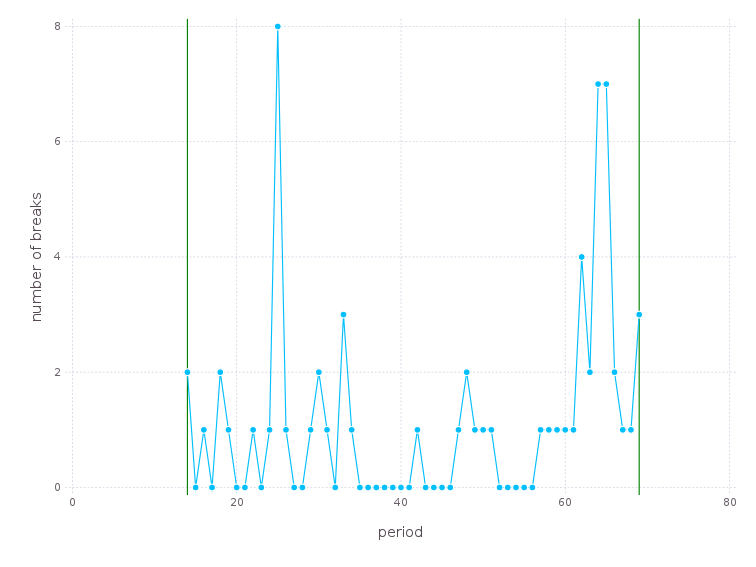
\includegraphics[width=8cm]{graphs/structural_breaks.png}}
\subfloat[1\% significance level]{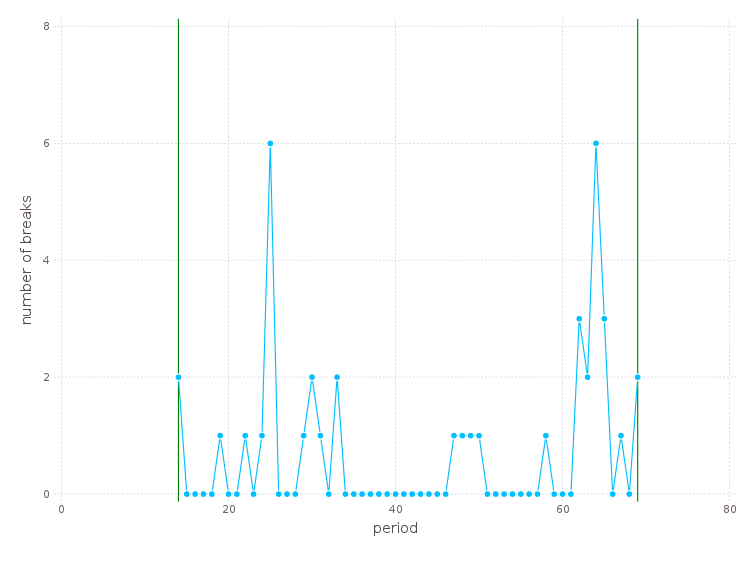
\includegraphics[width=8cm]{graphs/structural_breaks_1percent.png}}
\end{figure}

In the following the question of how to react to the presence of structural breaks is approached as in section 2 above. Either the length of the series is reduced by estimating the model only on data which is not subjected to structural breaks or the width of the data is reduced by removing the variables which are subjected to the structural break or a combination thereof. For the purpose of this paper we are interested in forecasting performance of factor models which ignore structural breaks versus factor models which take the structural breaks into account. Thus the results of models which restrict the amount of data to reduce the effect of structural breaks are compared with those that do not. It is worth noting that the comparison is not perfect because as has been argued in section $2$ it can be better to reduce the number of predictors to a set which is "targeted" towards the prediction of the variable of interest. It is possible that removing the variables with structural breaks "accidentally" targets the set of variables towards predicting the variable of interest independent of the structural break. In other words an improved result is not necessarily only due to the structural breaks being removed but might be due to a noisy predictor being removed. To be precise a series with a structural break could be considered a noisy predictor as well. However, it might be noisy independent of the structural breaks.
Resultingly, a robustness check consists of targeting the set of variables for both approaches prior to the estimation to remove that effect.

A practical difficulty has to be addressed before the results are presented. Given the fact that there are two periods where a majority of structural breaks occur, each of which affects a different set of factor loadings, cutting off the values before the significant break periods would leave very few observations for estimating the new model.

If both periods with major structural breaks are treated in a way that only data after the structural breaks is used, this would leave at most $17$ observations of which another $15$ have to be removed for the first step in the pseudo out-of-sample forecasts.

In principle there is a simple way to overcome this issue. It can be remembered that some of the data columns are monthly series which have been merged into the quarterly data set by dropping two thirds of the observations. The data could be cast back into monthly form. Most of the series will have missing data which can be interpolated (e.g. GDP is only reported quarterly). While this method solves the problem in a technical sense\footnote{For the first step of the pseudo out-of-sample period there are only $8$ data points for estimation. For every quarterly step of the pseudo out-of-sample procedure there are an additional $3$ observations. Thus, the ratio of observations to predictors improves quickly with each step of the pseudo out-of-sample prediction.}, it has several drawbacks: firstly no additional information is added by the interpolation although there are more observations available to the model. At the same time the imputation adds additional uncertainty. Traditional standard error estimates do not account for this and resultingly they may be downward biased (cf. \citet[chapter~25]{gelman2006missing}. It is thus likely that prediction based on this short data set performs badly in a forecasting sense. On the other hand, if predictions resulting from this shaved data set should perform better, it would constitute a strong indication that the structural breaks uncovered by the tests should not be ignored. In this case doing so clearly leads to a significant degradation of forecasting results. This has not been tested here. 

Instead four approaches to removing the effects of structural breaks from the data are considered. First the variables in the second cluster of structural breaks between the second quarter of 2008 and the first quarter of 2009 are removed. Because this approaches ignores the first cluster of structural breaks in the first quarter of 1999, a second model is estimated to explore what happens if these series are excluded as well. A third model removes all series with structural breaks in the loadings. Finally, the fourth model leaves the \textit{variables} with breaks in the first cluster in 1999 in the model but removes \textit{observations} prior to the second quarter of 1999. 

For all four approaches the best performing dynamic factor model in terms of RMSE is reported where the number of static factors in the factor equation is calculated using the IC$_{p2}$ criterion and the number of factors in the forecasting equation as well as the number of factor lags is chosen according to the minimum of the RMSE of out-of-sample forecasts. Structural breaks are detected at the $5\%$ significance level.

The figures in appendix \ref{structural breaks, reduced data sets} show the number of significant structural breaks left if the above adjustements to the data have been made. The reason to check for structural breaks again after some variables have been removed or the observations prior to the second quarter of 1999 have been removed, is that the estimation of the factor equation changes with a reduced set of variables which has an impact on the statistics of the structural break tests.

Table \ref{results dynamic factor model, reduced data sets} shows that the exclusion of variables improves the RMSE considerably compared to ignoring the structural breaks. For this data set, the more variables with structural breaks at the 5\% significance level are removed, the lower the RMSE becomes.

\begin{table}[ht]
	\centering
	\begin{tabular}{c|lllll}
		   & $r_{factor}$ & $r_{forecast}$ & $s$ & $q$ & RMSE\\
		 \hline
		 \hline
		  & \multicolumn{3}{c}{\textit{Second break cluster removed}} \\ 
			& & \multicolumn{3}{c}{$T=82, N=149$} \\
		  \hline
		   	RMSE & 7 & 7 & 1 & 3 & 0.45 \\
		   	RMSE \& $IC_{p2}$ & 3 & 7 & 1 & 3 & 0.45 \\
		  \hline
		  \hline
		  & \multicolumn{5}{c}{\textit{First and second break cluster removed}} \\ 
			& & \multicolumn{3}{c}{$T=82, N=141$} \\
		  \hline
		   	RMSE & 6 & 6 & 4 & 2 & 0.44 \\
		   	RMSE \& $IC_{p2}$ & 3 & 6 & 4 & 2 & 0.44 \\
		  \hline
		  \hline
	  	  & \multicolumn{5}{c}{\textit{All variables with breaks removed}} \\ 
			& & \multicolumn{3}{c}{$T=82, N=105$} \\
          \hline
		   	RMSE & 6 & 6 & 3 & 2 & 0.39 \\
		   	RMSE \& $IC_{p2}$ & 3 & 3 & 4 & 2 & 0.40 \\
		  \hline
		  \hline
		  & \multicolumn{5}{c}{\textit{Second break cluster removed, length trimmed}} \\
			& & \multicolumn{3}{c}{$T=57, N=149$} \\
		  \hline
		   	RMSE & 1 & 1 & 5 & 1 & 0.51 \\
		   	RMSE \& $IC_{p2}$ & 4 & 1 & 5 & 1 & 0.51 \\
		  \hline
		  \hline		  
	\end{tabular}
	\caption{Dynamic factor model, data adjusted for structural breaks}
	\label{results dynamic factor model, reduced data sets}
\end{table}


Figures for the number of structural breaks per period after variables have been dropped or the data length has been trimmed can be found in appendix \ref{structural breaks, reduced data sets}. Notably figure \ref{reduced data set, all variables with breaks removed} shows a modest number of structural breaks at the 5\% significance level although all structural breaks had been removed from the data set. Iterating the procedure by removing the variables with structural breaks again increases the RMSE to $0.72$ which makes clear that blindly removing all variables with structural breaks in them need not be a good idea although table \ref{results dynamic factor model, reduced data sets} indicates that removing as many variables with structural breaks as possible has a positive effect on RMSE.

\subsubsection{Targeted predictors}







\clearpage
\newpage
\appendix
\section*{Apendix}
\addcontentsline{toc}{section}{Appendix}

\section{Derrivation of Principal Components}
\label{Derrivation of Principal Components}
The principal components of a data matrix $X$ are defined as the transformation of $X$ into the space spanned by the loadings \footnote{The $u_i$ are also called scores or principal component directions.} $u_i$ where each $u_i$ is a unit vector. The transformation is defined such that the transformed columns are uncorrelated (as are the loadings $u_i$) and such that the first transformed column (i.e. the first principal component) contains the largest amount of the variance of the original data, the second column the second largest amount (i.e. the second principal component), etc. \\

Let $X$ have mean 0 (i.e. subtract the mean from each observation if it does not).
For the first principal component, we want to find a loading vector vector $u_1$ such that the variance along the projection of $x$ onto the first principal component direction $u_1$ is maximized where $u_1$ is a unit norm vector. 
$$\underset{u_1: ||u_1|| = 1}{\max} \ \frac{1}{T} \sum_{i=1}^T(x_i'u_1)^2 = \underset{u_1: u_1'u_1 = 1}{\max} \ u_1' ( \frac{1}{T} \sum_{i=1}^T x_i'x_i )u_1 = \underset{u_1: u_1'u_1 = 1}{\max} \ u_1' (\Sigma)u_1$$
Setting up the Lagrangian yields
$$ L(u_1, \lambda) = u_1' \Sigma u_1 - \lambda(u_1'u_1-1)$$
After taking the derivative with respect to $u_1$ and dividing by 2 we are left with
$$\frac{\partial L}{\partial u_1} = \Sigma u_1 -\lambda u_1 \overset{!}{=} 0$$ in other words $u_1$ is an eigenvector of $\Sigma$, the covariance matrix of x. The corresponding eigenvalue is $\lambda$ and we must have $\Sigma = \lambda$ for the variance of the principal component to be maximal under the constraint. \\
The maximal variance of $x'u_1$ is thus $V(x'u_1) = u_1' \Sigma u_1 = u_1' \lambda u_1$ and it is achieved for the highest eigenvalue $\lambda$ of the covariance matrix of x. The derrivation of the following principal components is accordingly subject to the additional constraint that the principal components are uncorrelated. In the case of the second principal component this implies $\text{cov}(u_1'x, u_2'x) = u_1' \Sigma u_2 = 0$. The solution for the third and all following principal component is more complex but goes accordingly. The derrivations can be seen e.g. in \citet{jolliffe2005principal} or any other textbook on the subject. The solution for the $i$-th principal component is to set the loadings $u_i$ to be eigenvector which belongs to the $i$-th highest eigenvalue. Also, for each principal component $i$ we get that $\text{var}(u_i'x) = \lambda_i$.

\newpage
\section{Estimation of the Factor Equation}
\label{Estimation of the Factor Equation}
Estimators of the factor equation solve (\ref{factor equation minimization problem}).
$$\min_{F_1, ..., F_T, \Lambda} V_r(\Lambda, F) = \min_{F_1, ..., F_T, \Lambda} \frac{1}{NT} \sum_{t=1}^T (X_t - \Lambda F_t)'(X_t - \Lambda F_t)$$

$$\text{s.t. } N^{-1} \Lambda' \Lambda = I_r$$

The solution can be gotten by first optimizing over $F_t$. The first order condition is: $$\frac{\partial V_r}{\partial F_t} = -2X'_t \Lambda + 2 \hat F'_t \Lambda' \Lambda \overset{!}{=} 0$$

Resultingly $\hat F_t = (\Lambda' \Lambda)^{-1} \Lambda' X_t$. Inserting that back into the optimization problem gives $\min_\Lambda \frac{1}{NT} X_t'X_t - 2X_t' \Lambda (\Lambda' \Lambda)^{-1} \Lambda'X_t + X_t' \Lambda (\Lambda' \Lambda)^{-1} \Lambda' \Lambda (\Lambda' \Lambda)^{-1} \Lambda'X_t = \min_\Lambda \frac{1}{NT} X_t' [I - \Lambda (\Lambda' \Lambda)^{-1} \Lambda']X_t$. \\
This is equivalent to the problem $\max_\Lambda \text{tr}\left\{(\Lambda'\Lambda)'^{-\frac{1}{2}}\lambda'(T^{-1} \Sigma_{t=1}^T X_tX_t') \Lambda (\Lambda' \Lambda)^{-\frac{1}{2}}\right\}$ which is the same as $\max_\Lambda \Lambda' \hat \Sigma_{XX} \Lambda \text{ s.t. } N^{-1} \Lambda' \Lambda = I_r$ where $\hat \Sigma_{XX}$ is the usual sample equivalent of the variance of $X$. This can be solved by setting $\hat \Lambda$ to eigenvectors of the $r$ largest eigenvalues of $\hat \Sigma_{XX}$.


\newpage
\section{Replication of \citet{bai2002determining} for $r=7$ and $r=9$}

\label{bai ng information criteria}
\begin{table}[h!]
\caption{Replication of Table I of \citet{bai2002determining} for $r=7$}
\center{
	DGP: $X_{it} = \sum_{j=1}^r \lambda_{ij}F_{tj} + \sqrt{\theta}e_{it}, r=7$
} \\

\center

\begin{tabular}{cc|lllllll}

	N & T & $PC_{p1}$ & $PC_{p2}$ & $PC_{p3}$ & $IC_{p1}$ & $IC_{p2}$ & $IC_{p3}$\\
	\hline
		100 & 40 & 6.4 & 5.9 & 6.97 & 4.93 & 3.46 & 6.73 & \\ 
		100 & 60 & 6.72 & 6.27 & 7.02 & 6.34 & 4.74 & 6.99 & \\ 
		200 & 60 & 6.93 & 6.87 & 7.0 & 6.78 & 6.46 & 6.96 & \\ 
		500 & 60 & 6.99 & 6.96 & 7.0 & 6.94 & 6.92 & 6.99 & \\ 
		1000 & 60 & 7.0 & 6.99 & 7.0 & 6.99 & 6.97 & 7.0 & \\ 
		2000 & 60 & 7.0 & 6.99 & 7.0 & 6.98 & 6.99 & 7.0 & \\ 
		100 & 100 & 7.0 & 6.77 & 7.35 & 6.89 & 6.32 & 50.0 & \\ 
		200 & 100 & 7.0 & 7.0 & 7.0 & 7.0 & 6.99 & 7.0 & \\ 
		500 & 100 & 7.0 & 7.0 & 7.0 & 7.0 & 7.0 & 7.0 & \\ 
		1000 & 100 & 7.0 & 7.0 & 7.0 & 7.0 & 7.0 & 7.0 & \\ 
		2000 & 100 & 7.0 & 7.0 & 7.0 & 7.0 & 7.0 & 7.0 & \\ 
		40 & 100 & 6.39 & 6.12 & 7.02 & 4.86 & 3.49 & 6.78 & \\ 
		60 & 100 & 6.79 & 6.37 & 7.01 & 6.01 & 5.0 & 7.0 & \\ 
		60 & 200 & 6.93 & 6.85 & 7.0 & 6.82 & 6.58 & 6.98 & \\ 
		60 & 500 & 6.96 & 6.97 & 7.0 & 6.97 & 6.9 & 6.99 & \\ 
		60 & 1000 & 7.0 & 6.99 & 7.0 & 6.99 & 6.96 & 7.0 & \\ 
		60 & 2000 & 7.0 & 7.0 & 7.0 & 6.97 & 6.98 & 6.99 & \\ 
		4000 & 60 & 7.0 & 7.0 & 6.99 & 6.98 & 6.99 & 6.99 & \\ 
		4000 & 100 & 7.0 & 7.0 & 7.0 & 7.0 & 7.0 & 7.0 & \\ 
		8000 & 60 & 6.99 & 7.0 & 7.0 & 7.0 & 6.98 & 7.0 & \\ 
		8000 & 100 & 7.0 & 7.0 & 7.0 & 7.0 & 7.0 & 7.0 & \\ 
		60 & 4000 & 7.0 & 7.0 & 7.0 & 7.0 & 7.0 & 6.99 & \\ 
		100 & 4000 & 7.0 & 7.0 & 7.0 & 7.0 & 7.0 & 7.0 & \\ 
		60 & 8000 & 6.99 & 7.0 & 7.0 & 6.99 & 7.0 & 6.99 & \\ 
		100 & 8000 & 7.0 & 7.0 & 7.0 & 7.0 & 7.0 & 7.0 & \\ 
	\hline
		10 & 50 & 5.0 & 5.0 & 5.0 & 4.76 & 3.95 & 5.0 & \\ 
		10 & 100 & 5.0 & 5.0 & 5.0 & 4.58 & 4.18 & 4.96 & \\ 
		20 & 100 & 7.04 & 6.5 & 7.98 & 3.14 & 2.07 & 6.94 & \\ 
		100 & 10 & 5.0 & 5.0 & 5.0 & 5.0 & 4.96 & 5.0 & \\ 
		100 & 20 & 7.1 & 6.64 & 8.05 & 3.3 & 2.08 & 8.2 & \\ 
	\hline
	\hline
	\\
	\multicolumn{8}{l} {\begin{minipage}{9.5cm}
		\small{\textbf{\textit{Notes:}} Estimated number of factors averaged over 1000 simulations. The true number of factors is $r$ and the maximum number of factors is $\text{ceil}(\min\{T, N\})/2)$.}
	\end{minipage}} \\

\end{tabular}
\end{table}

\begin{table}
\caption{Replication of Table I of \citet{bai2002determining} for $r=9$}
\center{
	DGP: $X_{it} = \sum_{j=1}^r \lambda_{ij}F_{tj} + \sqrt{\theta}e_{it}, r=9$
} \\
\center{
	see \citet{bai2002determining} for specification of the DGP
}

\center
\begin{tabular}{cc|lllllll}
	N & T & $PC_{p1}$ & $PC_{p2}$ & $PC_{p3}$ & $IC_{p1}$ & $IC_{p2}$ & $IC_{p3}$\\
	\hline
		100 & 40 & 6.51 & 5.93 & 8.06 & 3.55 & 1.49 & 7.89 & \\ 
		100 & 60 & 7.02 & 6.25 & 8.77 & 5.4 & 2.74 & 8.9 & \\ 
		200 & 60 & 7.74 & 7.31 & 8.65 & 7.33 & 6.26 & 8.74 & \\ 
		500 & 60 & 8.09 & 8.02 & 8.52 & 8.18 & 7.97 & 8.58 & \\ 
		1000 & 60 & 8.42 & 8.38 & 8.59 & 8.45 & 8.25 & 8.62 & \\ 
		2000 & 60 & 8.47 & 8.32 & 8.59 & 8.67 & 8.56 & 8.64 & \\ 
		100 & 100 & 8.03 & 6.93 & 9.01 & 7.68 & 4.85 & 50.0 & \\ 
		200 & 100 & 8.85 & 8.48 & 8.99 & 8.92 & 8.58 & 9.0 & \\ 
		500 & 100 & 9.0 & 8.99 & 9.0 & 9.0 & 8.99 & 9.0 & \\ 
		1000 & 100 & 9.0 & 8.99 & 9.0 & 9.0 & 9.0 & 9.0 & \\ 
		2000 & 100 & 9.0 & 9.0 & 9.0 & 9.0 & 9.0 & 9.0 & \\ 
		40 & 100 & 6.63 & 6.06 & 8.08 & 3.38 & 1.66 & 7.79 & \\ 
		60 & 100 & 7.03 & 6.33 & 8.85 & 5.51 & 2.68 & 8.94 & \\ 
		60 & 200 & 7.79 & 7.43 & 8.6 & 7.1 & 6.05 & 8.73 & \\ 
		60 & 500 & 8.16 & 7.98 & 8.61 & 8.28 & 7.96 & 8.66 & \\ 
		60 & 1000 & 8.41 & 8.28 & 8.51 & 8.51 & 8.34 & 8.69 & \\ 
		60 & 2000 & 8.4 & 8.4 & 8.58 & 8.57 & 8.56 & 8.74 & \\ 
		4000 & 60 & 8.52 & 8.44 & 8.57 & 8.61 & 8.51 & 8.73 & \\ 
		4000 & 100 & 9.0 & 9.0 & 9.0 & 9.0 & 9.0 & 9.0 & \\ 
		8000 & 60 & 8.44 & 8.52 & 8.55 & 8.66 & 8.64 & 8.68 & \\ 
		8000 & 100 & 9.0 & 9.0 & 9.0 & 9.0 & 9.0 & 9.0 & \\ 
		60 & 4000 & 8.53 & 8.54 & 8.55 & 8.62 & 8.6 & 8.57 & \\ 
		100 & 4000 & 9.0 & 9.0 & 9.0 & 9.0 & 9.0 & 9.0 & \\ 
		60 & 8000 & 8.61 & 8.47 & 8.51 & 8.66 & 8.58 & 8.76 & \\ 
		100 & 8000 & 9.0 & 9.0 & 9.0 & 9.0 & 9.0 & 9.0 & \\ 
	\hline
		10 & 50 & 5.0 & 5.0 & 5.0 & 4.66 & 3.29 & 5.0 & \\ 
		10 & 100 & 5.0 & 5.0 & 5.0 & 4.32 & 3.59 & 4.77 & \\ 
		20 & 100 & 7.25 & 6.84 & 8.1 & 1.76 & 1.28 & 7.21 & \\ 
		100 & 10 & 5.0 & 5.0 & 5.0 & 4.96 & 4.74 & 5.0 & \\ 
		100 & 20 & 7.37 & 7.02 & 8.28 & 1.92 & 1.25 & 8.89 & \\ 
	\hline
	\hline
	\\
	\multicolumn{8}{l} {\begin{minipage}{9.5cm}
		\small{\textbf{\textit{Notes:}} Estimated number of factors averaged over 1000 simulations. The true number of factors is $r$ and the maximum number of factors is $\text{ceil}(\min\{T, N\})/2)$.}
	\end{minipage}} \\
\end{tabular}
\end{table}

\newpage

\section{Reestimation of structural break tests after reducing data sets}
\label{structural breaks, reduced data sets}

\begin{figure}[htp]
	\centering
	\subfloat[5\% significance level]{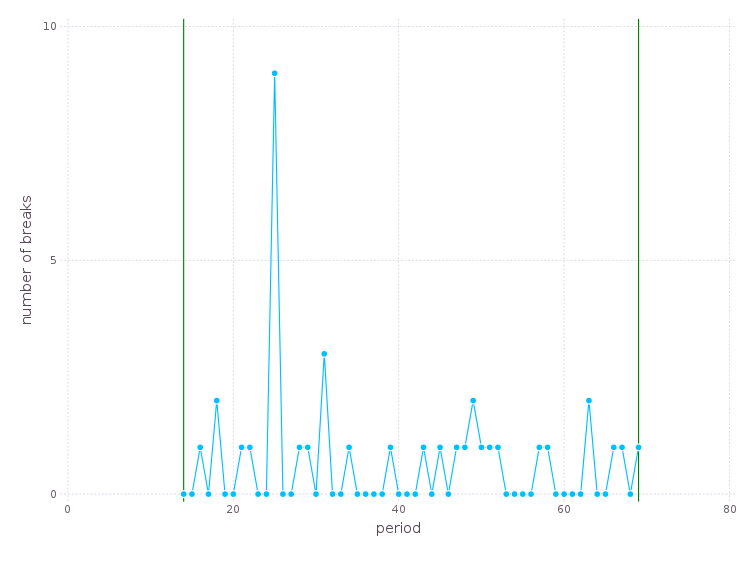
\includegraphics[width=8cm]{graphs/structural_breaks_less_variables.png}}
	\subfloat[1\% significance level]{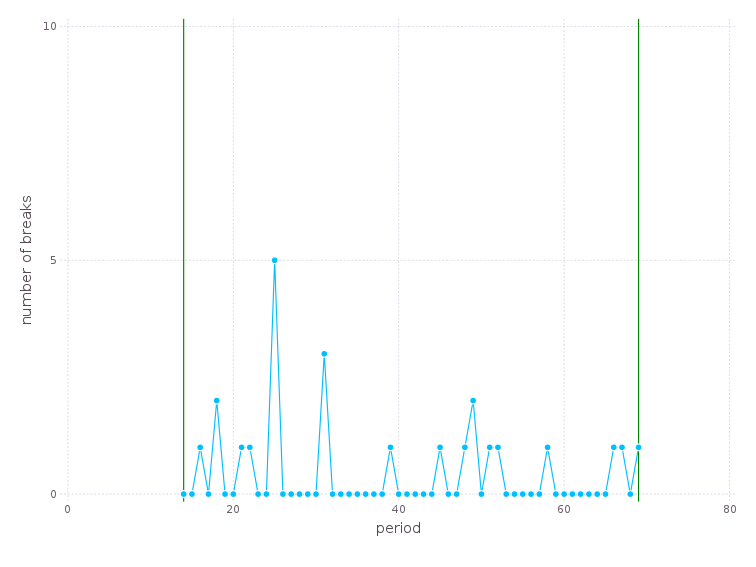
\includegraphics[width=8cm]{graphs/structural_breaks_less_variables_1percent.png}}
	\caption{Second cluster removed}
	\label{reduced data set, second cluster removed}
\end{figure}
	
\begin{figure}[htp]
	\subfloat[5\% significance level]{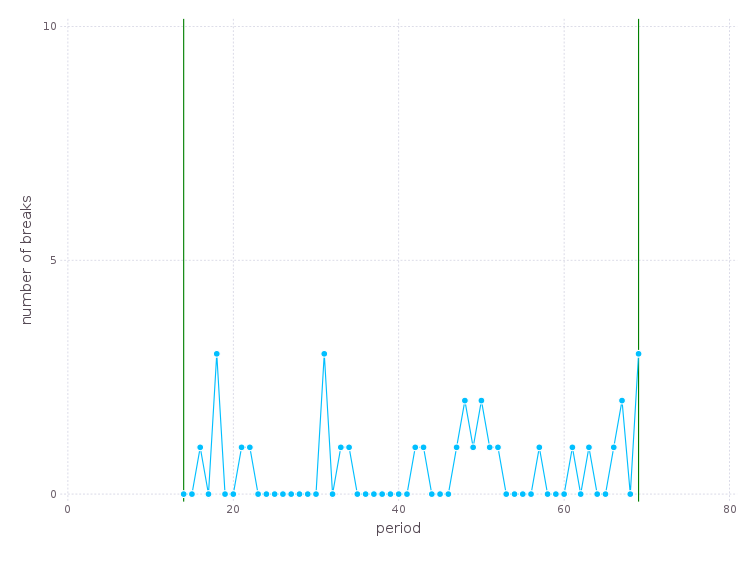
\includegraphics[width=8cm]{graphs/structural_breaks_even_less_variables.png}}
	\subfloat[1\% significance level]{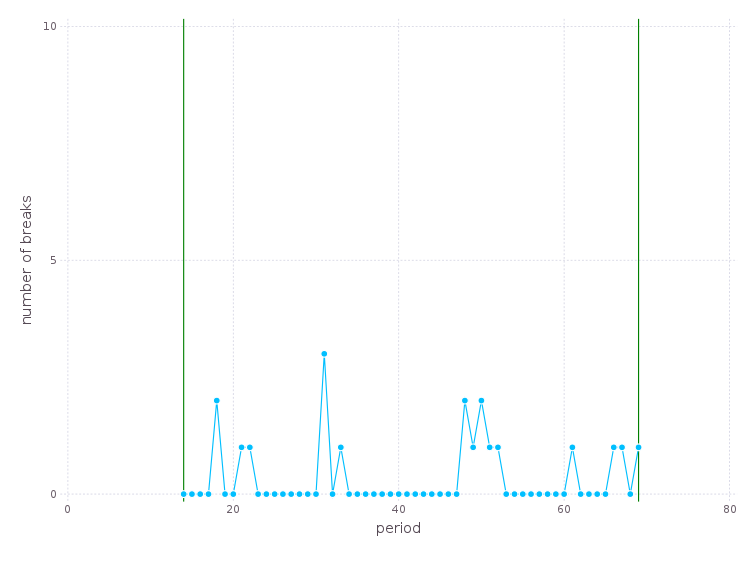
\includegraphics[width=8cm]{graphs/structural_breaks_even_less_variables_1percent.png}}
	\caption{First and second cluster removed}
	\label{reduced data set, first and second cluster removed}
\end{figure}

\begin{figure}[htp]
	\centering
	\subfloat[5\% significance level]{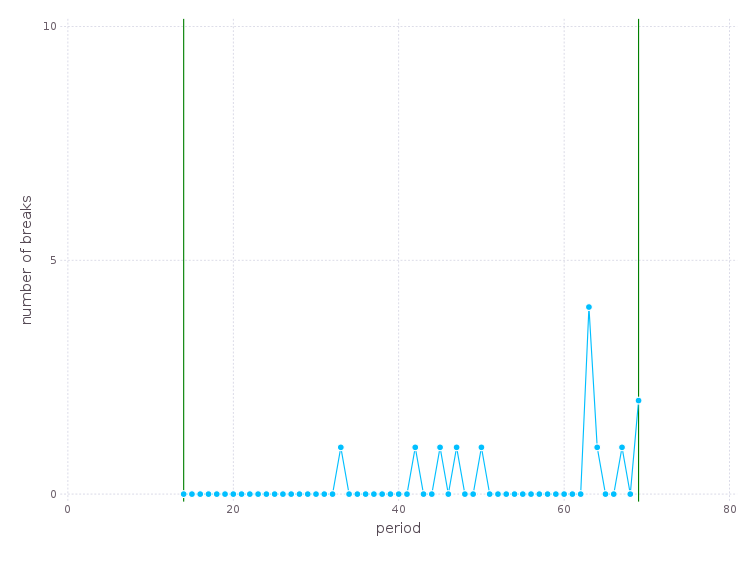
\includegraphics[width=8cm]{graphs/structural_breaks_all_breaks_removed.png}}
	\subfloat[1\% significance level]{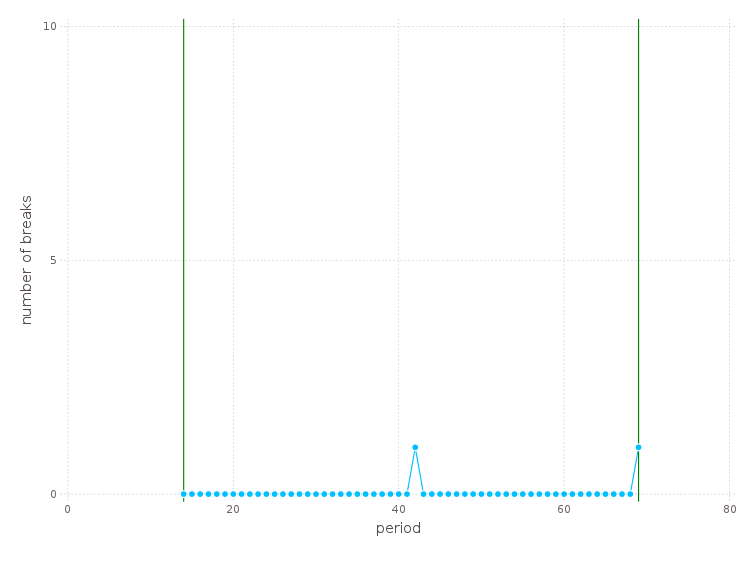
\includegraphics[width=8cm]{graphs/structural_breaks_all_breaks_removed_1percent.png}}
	\caption{All variables with breaks removed}
	\label{reduced data set, all variables with breaks removed}
\end{figure}

\begin{figure}[htp]
	\centering
	\subfloat[5\% significance level]{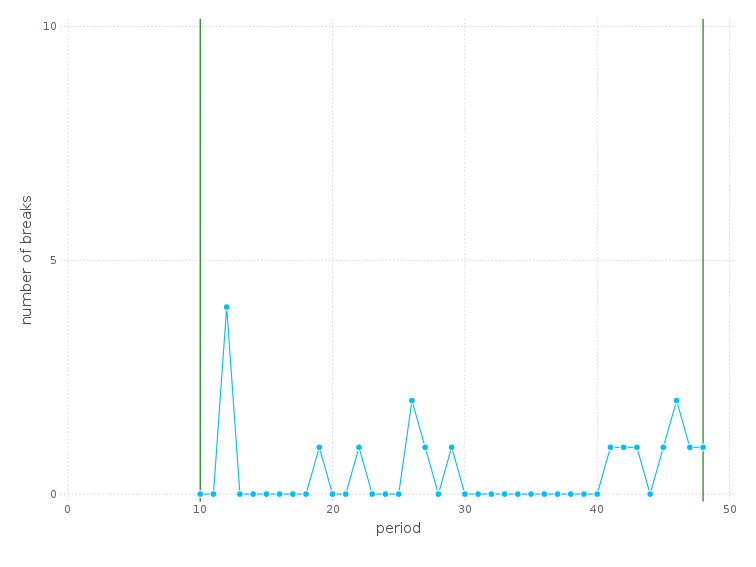
\includegraphics[width=8cm]{graphs/structural_breaks_second_cluster_and_obs_removed.png}}
	\subfloat[1\% significance level]{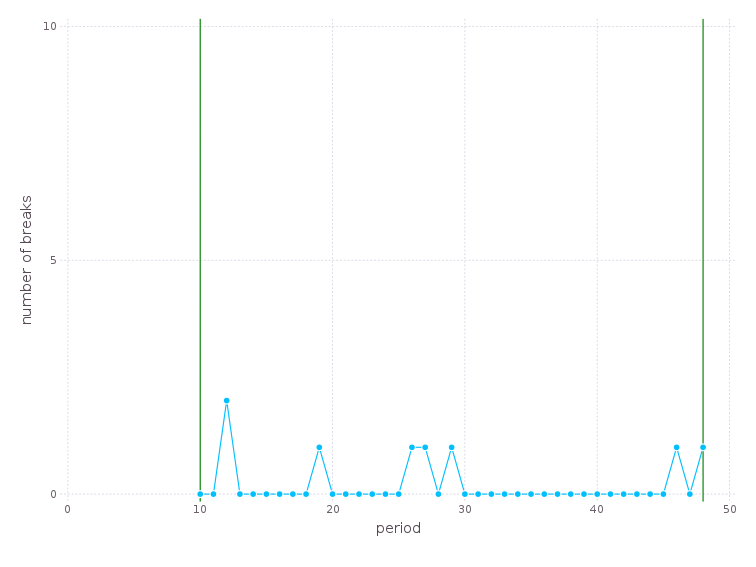
\includegraphics[width=8cm]{graphs/structural_breaks_second_cluster_and_obs_removed_1percent.png}}
	\caption{Second cluster removed, data set trimmed before 1991 quarter 1}
	\label{reduced data set, second cluster removed, data set trimmed}
\end{figure}



\clearpage
\newpage
\section{Data series}
\label{Data series}

\begin{table}[ht]
\label{Bundesbank data series}
\caption{Bundesbank data series}
\centering
\begin{tabular}{rp{5cm}p{11cm}}
& \textbf{Series Id} & \textbf{Series Title} \\
  \hline
  \hline
1 & BBNA2.Q.DE.N.I. 021.CA.D.V.I05.A, & Actual earnings/ Overall economy/ Wages and salaries per employee (workplace concept)/ Index/ Germany \\ 
  \hline
  2 & BBK01.EA4220, & Balance on current account \\ 
  \hline
  3 & BBK01.DU7834, & Basic pay rates, overall economy, excluding ancillary benefits, excluding one-off payments, on a monthly basis, Germany \\ 
  \hline
  4 & BBXS1.A.I7.N.EUBUCS. MANU.MAN013.TT.PCT.I00 & Business and consumer surveys (European Commission) / Capacity utilization (man) / Euro area 18 (fixed composition) \\ 
  \hline
  5 & BBXS1.A.DE.N.EUBUCS. MANU.MAN013.TT.PCT.I00 & Business and consumer surveys (European Commission) / Capacity utilization (man) / Germany \\ 
  \hline
  6 & BBK01.OU7744, & Capital / Total / All categories of banks \\ 
  \hline
  7 & BBK01.BQ1351, & Central government debt - total debt \\ 
  \hline
  8 & BBDE1.M.DE.Y.JAA9. P2XF50500.CB.V.ABA.A & Construction permits - estimated construction cost / At current prices, flows / Germany / Total (including construction work on existing buildings) - residential and non-residential buildings, total \\ 
  \hline
  9 & BBXR1.M.HWWI.N.EURO. TOTNXNGY.INDBEU.HE.M00 & Construction price index / Germany / Unadjusted figure / Total \\ 
  \hline
  10 & BBK01.OXA8R3 & domestic Financial Vehicle Corporations - All categories of banks \\ 
  \hline
  11 & BBDP1.M.DE.Y.VPI. C.A00000.I10.L & Consumer price index / Germany / Unadjusted figure / Total \\ 
  \hline
  12 & BBK01.WX9141 & DAX price index / End 1987 = 1000 / End of month \\ 
  \hline
  13 & BBK01.WT4065 & DE0001102358 / Prices / 1,500 Bund 14/24 \\ 
  \hline
  14 & BBK01.SUD106S & Effective interest rates of German banks / New business (estimated) / Households' deposits, overnight \\ 
  \hline
  15 & BBK01.SUD210 & Effective interest rates of German banks / New business / Non-financial corporations' deposits, overnight \\ 
  \hline
  16 & BBDE1.M.DE.Y.GUA1. P2XF13020.BA.V.ABA.A & Employed persons (including proprietors and family workers) / Persons / Germany / Main construction industry \\ 
  \hline
  17 & BBK01.US8CA0 & Employees subject to social security contributions / Total / Eastern Germany \\ 
  \hline
  18 & BBK01.US80CA & Employees subject to social security contributions / Total / Western Germany \\ 
\end{tabular}
\end{table}

\begin{table}
\centering
\begin{tabular}{rp{5cm}p{11cm}}
  & \textbf{Series Id} & \textbf{Series Title} \\
  \hline
  \hline

  19 & BBK01.USCA80 & Employment in Germany / Employed persons in Germany / Germany \\ 
  \hline
  20 & BBK01.JAB938 & Enterprises \\ 
  \hline
  21 & BBXN1.A.I7.N.NAG. B1QG00.0000.Z0N.IND.I00 & Euro area 18 (fixed composition) / National accounts - Gross domestic product / Gross domestic product / Total / Indices \\ 
  \hline
  22 & BBK01.XS5609, & Exports / European countries \\ 
  \hline
  23 & BBK01.XX3382, & Exports of the Federal Republic of Germany / Special Trade / Total / 1 / 2 / \\ 
  \hline
  24 & BBK01.EU4370, & Financial transactions / Other investment / Balance \\ 
  \hline
  25 & BBK01.EU2518, & Foreign investment in Germany / Other investment / Total / Balance \\ 
  26 & BBK01.EU4510 & Foreign trade / Exports (fob) \\ 
  \hline
  27 & BBMF1.M.D0.EUR. GOVT.WYWG.Y10.BID & Geldmenge M1 /                                                   Veränderung saisonbereinigt / Jahresrate / EWU \\ 
  \hline
  28 & BBK01.BQ2190 & General government budgetary position (Germany) - total revenue \\ 
  \hline
  29 & BBK01.BQM403 & General government debt - of which currency and deposits \\ 
  30 & BBK01.BQM208 & General government debt - of which loans \\ 
  \hline
  31 & BBK01.BQ8068 & General government debt as defined in the Maastricht Treaty - Germany - overall \\ 
  \hline
  32 & BBK01.BJ8072 & General government deficit / surplus as defined in the Maastricht Treaty - Germany - overall \\ 
  \hline
  33 & BBK01.XS4204 & German exports / special trade / values / 1 / 2 / 3 / 4 \\ 
  \hline
  34 & BBK01.XS4206 & German foreign trade balance / special trade / values / 1 / 2 / 3 / 4 \\ 
  \hline
  35 & BBK01.XS4205 & German imports / special trade / values / 1 / 2 / 3 / 4 \\ 
  \hline
  36 & BBK01.EC7750 & German investment abroad / EU member states (28) / Total / Balance \\ 
  \hline
  37 & BBK01.ED9065 & German investment abroad / Emerging markets and developing countries / Total / Balance \\ 
  \hline
  38 & BBK01.ED9004 & German investment abroad / Euro-area member states / Total / Balance \\ 
  \hline
  39 & BBK01.ED9001 & German investment abroad / Europe / Total / Balance \\ 
  \hline
  40 & BBK01.ED1096 & German investment abroad / Other EU member states / Total / Balance \\   
  \hline
  41 & BBK01.ED9031 & German investment abroad / Other European countries / Total / Balance \\ 
  \hline
  42 & BBK01.JBA161 & Gross domestic product / at current prices / Seasonally and working-day adjusted \\ 
  \hline
  43 & BBK01.JAA026 & Gross national income (GNP) / at current prices \\ 
  \hline
  44 & BBK01.WU0042 & Gross sales of domestic debt securities at nominal value / Total \\ 
  \hline
  45 & BBK01.JAA327 & Gross wages and salaries \\ 
  \hline
  46 & BBXP1.M.U2.N.HICP. 000000.IND.I00 & Hamonized Index of Consumer Prices / Euro area (changing composition) / Overall index / Unadjusted figure / Monthly \\ 
  \hline
  47 & BBK01.TQ7162 & Households - Household debt to GDP FSI-I033 \\ 
  \hline
  48 & BBK01.XS8953 & Imports / Product Classification for Production / Statistics from 2009 Total excluding energy \\ 
\end{tabular}
\end{table}

\begin{table}
\centering
\begin{tabular}{rp{5cm}p{11cm}}
& \textbf{Series Id} & \textbf{Series Title} \\
  \hline
  \hline
  49 & BBK01.XS8857 & Imports / Value / Total, excluding energy \\ 
  \hline
  50 & BBK01.EU4169 & Income / Total / Receipts \\ 
  \hline
  51 & BBDE1.Q.DE.Y.LCB1. A2N200000.A.L.I08.A1 & Index of gross wages and salaries / Germany / Mining and quarrying, manufacturing and service activities (B-S) \\ 
  \hline
  52 & BBDE1.Q.DE.Y.LCA1. A2N200000.A.L.I08.A1 & Index of labour costs / Germany / Mining and quarrying, manufacturing and service activities (B-S) \\ 
  \hline
  53 & BBDE1.Q.DE.Y.LCC1. A2N200000.A.L.I08.A1 & Index of non-wage costs / Germany / Mining and quarrying, manufacturing and service activities (B-S) \\ 
  \hline
  54 & BBDP1.M.DE.Y. VPI.C.SVXR.I10.A & Index of producer prices of industrial products sold on the domestic market / Germany \\ 
  \hline
  55 & BBEE1.M.DE.AAA. XY0U12.R.AACPB.M00 & Indicator of the German economy's price competitiveness against 24 selected industrial countries, based on the deflators of total sales \\ 
  \hline
  56 & BBK01.XSC430 & Indices of foreign trade prices - exports, total / Germany \\ 
  \hline
  57 & BBXE1.M.I7.W. PROD.NS0020.IND.I00 & Industrieproduktion / Gesamte Industrie (ohne Baugewerbe) / Index / nur kalenderbereinigt / Euro-Währungsgebiet-18 \\ 
  \hline
  58 & BBK01.EB0057 & International Investment Position, all countries, net, total (from end 1997) \\ 
  \hline
  59 & BBK01.OEAA56G & Kredite an Nichtbanken (Nicht-MFIs) / Nichtbanken (Nicht-MFIs) insgesamt / Kredite insgesamt / Baden-Württemberg \\ 
  \hline
  60 & BBK01.OEAA21H & Kredite an Nichtbanken (Nicht-MFIs) / Nichtbanken (Nicht-MFIs) insgesamt / Kredite insgesamt / Bayern \\ 
  \hline
  61 & BBK01.OEAA03I & Kredite an Nichtbanken (Nicht-MFIs) / Nichtbanken (Nicht-MFIs) insgesamt / Kredite insgesamt / Berlin \\ 
  \hline
  62 & BBK01.OEAA52S & Kredite an Nichtbanken (Nicht-MFIs) / Nichtbanken (Nicht-MFIs) insgesamt / Kredite insgesamt / Brandenburg \\ 
  \hline
  63 & BBK01.OEAA56J & Kredite an Nichtbanken (Nicht-MFIs) / Nichtbanken (Nicht-MFIs) insgesamt / Kredite insgesamt / Bremen \\ 
  \hline
  64 & BBK01.OEAA01K & Kredite an Nichtbanken (Nicht-MFIs) / Nichtbanken (Nicht-MFIs) insgesamt / Kredite insgesamt / Hamburg \\ 
  \hline
  65 & BBK01.OEAA56L & Kredite an Nichtbanken (Nicht-MFIs) / Nichtbanken (Nicht-MFIs) insgesamt / Kredite insgesamt / Hessen \\ 
  \hline
  66 & BBK01.OEAA37R & Kredite an Nichtbanken (Nicht-MFIs) / Nichtbanken (Nicht-MFIs) insgesamt / Kredite insgesamt / Mecklenburg-Vorpommern \\ 
  \hline
  67 & BBK01.OEAA56M & Kredite an Nichtbanken (Nicht-MFIs) / Nichtbanken (Nicht-MFIs) insgesamt / Kredite insgesamt / Niedersachsen \\ 
  \hline
  68 & BBK01.OEAA56N & Kredite an Nichtbanken (Nicht-MFIs) / Nichtbanken (Nicht-MFIs) insgesamt / Kredite insgesamt / Nordrhein-Westfalen \\ 
  \hline
  69 & BBK01.OEAA03O & Kredite an Nichtbanken (Nicht-MFIs) / Nichtbanken (Nicht-MFIs) insgesamt / Kredite insgesamt / Rheinland-Pfalz \\ 
  \hline
  70 & BBK01.OEAA03P & Kredite an Nichtbanken (Nicht-MFIs) / Nichtbanken (Nicht-MFIs) insgesamt / Kredite insgesamt / Saarland \\ 
  \hline
  71 & BBK01.OEAA56V & Kredite an Nichtbanken (Nicht-MFIs) / Nichtbanken (Nicht-MFIs) insgesamt / Kredite insgesamt / Sachsen \\ 
  \hline
  72 & BBK01.OEAA02T & Kredite an Nichtbanken (Nicht-MFIs) / Nichtbanken (Nicht-MFIs) insgesamt / Kredite insgesamt / Sachsen-Anhalt \\ 

 \end{tabular}
\end{table}
\begin{table}
\centering
\begin{tabular}{rp{5cm}p{11cm}}  
& \textbf{Series Id} & \textbf{Series Title} \\
  \hline
  \hline

  73 & BBK01.OEAA56Q & Kredite an Nichtbanken (Nicht-MFIs) / Nichtbanken (Nicht-MFIs) insgesamt / Kredite insgesamt / Schleswig-Holstein \\ 
  \hline
  74 & BBK01.OEAA56U & Kredite an Nichtbanken (Nicht-MFIs) / Nichtbanken (Nicht-MFIs) insgesamt / Kredite insgesamt / Thüringen \\ 
  \hline
  75 & BBK01.OEAB01G & Kredite an Nichtbanken (Nicht-MFIs) / insgesamt /  zusammen / Alle Bankengruppen / Baden-Württemberg \\ 
  \hline
  76 & BBK01.OEBB21H & Kredite an Nichtbanken (Nicht-MFIs) / insgesamt / zusammen / Alle Bankengruppen / Bayern \\ 
  \hline
  77 & BBK01.OEAB01I & Kredite an Nichtbanken (Nicht-MFIs) / insgesamt / zusammen / Alle Bankengruppen / Berlin \\ 
  \hline
  78 & BBK01.OEAB01S & Kredite an Nichtbanken (Nicht-MFIs) / insgesamt / zusammen / Alle Bankengruppen / Brandenburg \\ 
  \hline
  79 & BBK01.OEAB01J & Kredite an Nichtbanken (Nicht-MFIs) / insgesamt / zusammen / Alle Bankengruppen / Bremen \\ 
  \hline
  80 & BBK01.OEBB12K & Kredite an Nichtbanken (Nicht-MFIs) / insgesamt / zusammen / Alle Bankengruppen / Hamburg \\ 
  \hline
  81 & BBK01.OELB02L & Kredite an Nichtbanken (Nicht-MFIs) / insgesamt / zusammen / Alle Bankengruppen / Hessen \\ 
  \hline
  82 & BBK01.OEAB01R & Kredite an Nichtbanken (Nicht-MFIs) / insgesamt / zusammen / Alle Bankengruppen / Mecklenburg-Vorpommern \\ 
  \hline
  83 & BBK01.OEAB01M & Kredite an Nichtbanken (Nicht-MFIs) / insgesamt / zusammen / Alle Bankengruppen / Niedersachsen \\ 
  \hline
  84 & BBK01.OEAB01N & Kredite an Nichtbanken (Nicht-MFIs) / insgesamt / zusammen / Alle Bankengruppen / Nordrhein-Westfalen \\ 
  \hline
  85 & BBK01.OELB03O & Kredite an Nichtbanken (Nicht-MFIs) / insgesamt / zusammen / Alle Bankengruppen / Rheinland-Pfalz \\ 
  \hline
  86 & BBK01.OEAB01P & Kredite an Nichtbanken (Nicht-MFIs) / insgesamt / zusammen / Alle Bankengruppen / Saarland \\ 
  \hline
  87 & BBK01.OEYB19V & Kredite an Nichtbanken (Nicht-MFIs) / insgesamt / zusammen / Alle Bankengruppen / Sachsen \\ 
  \hline
  88 & BBK01.OEAB01T & Kredite an Nichtbanken (Nicht-MFIs) / insgesamt / zusammen / Alle Bankengruppen / Sachsen-Anhalt \\ 
  \hline
  89 & BBK01.OEAB01Q & Kredite an Nichtbanken (Nicht-MFIs) / insgesamt / zusammen / Alle Bankengruppen / Schleswig-Holstein \\ 
  \hline
  90 & BBK01.OEAB01U & Kredite an Nichtbanken (Nicht-MFIs) / insgesamt / zusammen / Alle Bankengruppen / Thüringen \\ 
  \hline
  91 & BBK01.SU0009 & Lending rates of banks / Current account credit less than EUR 100,000 / Average interest rate \\ 
  \hline
  92 & BBK01.SU0511 & Lending rates of banks / Long-term fixed-rate loans to enterprises and self-employed persons, EUR 100,000 and more but less than EUR 500,000, effective interest rate / Average interest rate \\ 
  \hline
  93 & BBK01.SU0012 & Lending rates of banks / Mortgage loans secured by residential real estate with interest rates fixed for 2 years, effective interest rate / Average interest rate \\ 
  \hline
  94 & BBK01.OU7677 & Lending to banks (MFIs) / Balances and loans / All categories of banks \\ 
\end{tabular}
\end{table}

\begin{table}
\centering
\begin{tabular}{rp{5cm}p{11cm}}
& \textbf{Series Id} & \textbf{Series Title} \\
  \hline
  \hline
  95 & BBK01.OU7676 & Lending to banks (MFIs) / Total / All categories of banks \\ 
  \hline
  96 & BBK01.PC3767 & Lending to computer and related activities, research and development / Total / All categories of banks \\ 
  \hline
  97 & BBK01.PC3723 & Lending to construction / Total/ All categories of banks \\ 
  \hline
  98 & BBK01.OU7712 & Lending to domestic banks (MFIs) / Credit balances and loans / All categories of banks \\ 
  \hline
  99 & BBK01.TUD364 & MONEY STOCK M1 (FROM 2002, EXCLUDING CURRENCY IN CIRCULATION) / GERMAN CONTRIBUTION \\ 
  \hline
  100 & BBK01.TQ7036 & Market liquidity - Average bid-ask spread in the securities market - government bills                          FSI-I035 \\ 
  \hline
  101 & BBK01.OU8045 & Medium and long-term lending / to general government / Securities / All categories of banks \\ 
  \hline
  102 & BBK01.OU8041 & Medium and long-term lending to general government / Loans / Long-term / All categories of banks \\ 
  \hline
  103 & BBK01.OU9829 & Medium and long-term lending to general government / Loans / Medium-term / All categories of banks \\ 
  \hline
  104 & BBK01.TS1303 & Monetary aggregate M3 (from January 2002, excluding currency in circulation; from June 2010, excluding repos with central counterparties) / German contribution / Outstanding amounts at the end of the month (stocks) \\ 
  \hline
  105 & BBK01.OUP001 & Money market paper issued by banks (MFIs) / All categories of banks \\ 
  \hline
  106 & BBK01.SU0295 & Money market rates / EONIA / Monthly average \\ 
  \hline
  107 & BBK01.SU0334G & Money market rates / EURIBOR three-month funds / Moving monthly average \\ 
  \hline
  108 & BBK01.TVE309 & Money stock M3 / EMU / Total / Changes \\ 
  \hline
  109 & BBK01.JB5001 & National accounts - domestic demand (price adjusted) \\ 
  \hline  110 & BBK01.JB5007 & National accounts - employment / Germany / 1 / 2 / \\ 
  \hline
  111 & BBK01.JB5005 & National accounts - exports (price adjusted) / \\ 
  \hline
  112 & BBK01.JQ5003 & National accounts - government consumption (price adjusted) \\ 
  \hline
  113 & BBK01.JB5004 & National accounts - gross fixed capital formation (price adjusted) \\ 
  \hline
  114 & BBK01.JB5008 & National accounts - labour costs per employee / \\ 
  \hline
  115 & BBK01.JQ5002 & National accounts - private consumption (price adjusted) \\ 
  \hline
  116 & BBK01.BJ9195 & National accounts - total general government revenue (ESA 95) - Germany as a whole (western Germany up to and including 1990) \\ 
  \hline
  117 & BBK01.BJ9049 & National accounts - total general government revenue (GFS as defined by the ECB) - Germany as a whole \\ 
  \hline
  118 & BBNA2.Q.DE.N.I. 041.CA.D.V.I05.A & National accounts / Gross wages and salaries per hour worked by employees /  Whole economy / Germany \\ 
  \hline
  119 & BBK01.JJA327 & National accounts/Households' income/Germany/ Gross wages and salaries (residence concept) \\ 
  \hline
  120 & BBK01.JQA024 & National accounts/Labour productivity per hour worked by persons in employment/ Whole economy \\ 
  \hline
  121 & BBK01.JJB071 & National accounts/Origin of GDP/Chain-linked index/ Production sector (excluding construction) \\ 
\end{tabular}
\end{table}

\begin{table}
\centering
\begin{tabular}{rp{5cm}p{11cm}}
& \textbf{Series Id} & \textbf{Series Title} \\
  \hline
  \hline
  122 & BBK01.JQA001 & National accounts/Overall economic view/ Compensation of employees - residents \\ 
  \hline
  123 & BBK01.JQC000 & National accounts/Overall economic view/At current prices/ GDP \\ 
  \hline
  124 & BBK01.JJB949 & National accounts/Unit labour costs per hour/ Whole economy (excluding agriculture, forestry and fishing, public services, education and health and other services) \\ 
  \hline
  125 & BBK01.JQA111 & National accounts/Use of GDP/At current prices/ Private consumption \\ 
  \hline
  126 & BBK01.JQC111 & National accounts/Use of GDP/Price index/ Private consumption \\ 
  \hline
  127 & BBK01.OXA8T5 & off-balance true sale of domestic banks (MFIs) - All categories of banks \\ 
  \hline
  128 & BBEE1.A.I7.AAA. XZE021.R.AACPE.M00 & Nominal effective exchange rate of the euro against the currencies of the EER-20 group \\ 
  \hline
  129 & BBK01.TQ7032 & Non-financial corporations sector - Total debt to equity FSI-I028 \\ 
  \hline
  130 & BBDE1.M.DE.Y.AEA1. A2P300000.F.C.I10.L & Orders received / At constant prices / Germany / Industry / Unadjusted figure \\ 
  \hline
  131 & BBDE1.M.DE.Y.AEA1. P2XF04000.B2.C.I10.A & Orders received / At constant prices / Germany / Main construction industry \\ 
  \hline
  132 & BBDE1.M.DE.W.AEA1. A2P340000.F.V.I10.A & Orders received / At current prices / Germany / Industry / Calendar adjusted only \\ 
  \hline
  133 & BBDE1.M.DE.Y.AEA1. A2P300000.F.C.I10.A & Orders received / At current prices / Germany / Industry \\ 
  \hline
  134 & BBDE1.M.DE.Y.AEA1. A2Q501000.F.V.I10.A & Orders received / At current prices, flows / Germany / 20+21 Manufacture of chemicals, chemical products; basic pharmaceutical products and pharmaceutical preparations \\ 
  \hline
  135 & BBDE1.M.DE.W.AEA1. P2XF04000.B2.V.I10.A & Orders received / At current prices, flows / Germany / Main construction industry / Calendar adjusted only \\ 
  \hline
  136 & BBDE1.M.DE.Y.AEA1. P2XF13010.B2.V.I10.A & Orders received / At current prices, flows / Germany / Main construction industry \\ 
  \hline
  137 & BBDE1.M.DE.W.AEN1. A2P340000.F.V.I10.A & Orders received excluding large orders, domestic / At current prices, flows / Germany / Industry / Calendar adjusted only \\ 
  \hline
  138 & BBDE1.M.DE.Y.AEN1. A2P350000.F.C.I10.A & Orders received excluding large orders, domestic / At current prices, flows / Germany / Industry  \\ 
  \hline
  139 & BBDE1.M.DE.Y.AEP1. A2P350000.F.C.I10.A & Orders received excluding large orders, euro-area countries / At current prices, flows / Germany / Industry \\ 
  \hline
  140 & BBDE1.M.DE.W.AEN5. A2P340000.F.V.I10.A & Orders received excluding large orders, foreign / At current prices, flows / Germany / Industry / Calendar adjusted only \\ 
  \hline
  141 & BBDE1.M.DE.Y.AEN5. A2P350000.F.C.I10.A & Orders received excluding large orders, foreign / At current prices, flows / Germany / Industry \\ 
  \hline
  142 & BBDE1.M.DE.Y.AEP5. A2P350000.F.C.I10.A & Orders received excluding large orders, non-euro-area countries / At current prices, flows / Germany / Industry \\ 
  \hline
  143 & BBDE1.M.DE.W.AEM1. A2P340000.F.V.I10.A & Orders received excluding large orders, total / At current prices, flows / Germany / Industry / Calendar adjusted only \\ 
  \hline
  144 & BBDE1.M.DE.Y.AEM1. A2P350000.F.C.I10.A & Orders received excluding large orders, total / At current prices, flows / Germany / Industry \\ 

\end{tabular}
\end{table}

\begin{table}
\centering
\begin{tabular}{rp{5cm}p{11cm}}
& \textbf{Series Id} & \textbf{Series Title} \\
  \hline
  \hline
  145 & BBDE1.M.DE.Y.AEB5. A2P350000.F.C.I10.A & Orders received from abroad / At current prices / Germany / Industry \\ 
  \hline
  146 & BBDE1.M.DE.Y.AEB1. A2Q501000.F.C.I10.A & Orders received from the domestic market / At constant prices / Germany / 20+21 Manufacture of chemicals, chemical products; basic pharmaceutical products and pharmaceutical preparations \\ 
  \hline
  147 & BBDE1.M.DE.Y.AEB1. A2P350000.F.C.I10.A & Orders received from the domestic market / At current prices / Germany / Industry \\ 
  \hline
  148 & BBDE1.M.DE.Y.BAA1. P2XF00000.G.C.I10.L & Output in the production sector / At constant prices / Germany / Main construction industry / Unadjusted figure \\ 
  \hline
  149 & BBDE1.M.DE.Y.BAA1. A2P300000.G.C.I10.A & Output in the production sector / Germany / Production sector including construction (B -F) \\ 
  \hline
  150 & BBEX3.M.XAU. DEM.EA.AC.C02, & Price of gold in London / morning fixing * / 1 ounce of fine gold = USD ... \\ 
  \hline
  151 & BBDE1.M.DE.Y.FG30. A2P200000.F.N.I10.A & Produktionsergebnis je Beschäftigten / Deutschland / Bergbau und Gewinnung von Steinen und Erden sowie Verarbeitendes Gewerbe (B + C) / Angaben für fachliche Betriebsteile / kalender- und saisonbereinigt \\ 
  \hline
  152 & BBK01.TQ7040 & Real estate markets - Residential real estate loans to total loans                                        FSI-I039 \\ 
  \hline
  153 & BBK01.TXI362 & TOTAL ASSETS OR LIABILITIES / GERMAN CONTRIBUTION \\ 
  \hline
  154 & BBK01.TUB618 & Total assets \\ 
  \hline
  155 & BBK01.TUE365 & Total assets or liabilities / Euro area \\ 
  \hline
  156 & BBK01.TUB641 & Total liabilities \\ 
  \hline
  157 & BBK01.UJCY01 & Unemployment rate (unemployment as a percentage of the civilian labour force) / Germany \\ 
\end{tabular}
\end{table}



\begin{table}
\centering
\label{FRED data series}
\caption{FRED data series}
\begin{tabular}{rp{5cm}p{11cm}}
	& \textbf{Series Id} & \textbf{Series Title} \\
  \hline
  \hline
	158 & A229RX0 & Real Disposable Personal Income: Per capita \\
  \hline
	159 & AAA & Moody's Seasoned Aaa Corporate Bond Yield© \\
  \hline
	160 & AHECONS & Average Hourly Earnings Of Production And Nonsupervisory Employees: Construction \\
  \hline
	161 & AHEMAN & Average Hourly Earnings Of Production And Nonsupervisory Employees: Manufacturing \\
  \hline
	162 & AWHMAN & Average Weekly Hours of Production and Nonsupervisory Employees: Manufacturing \\ 
  \hline
	163 & AWOTMAN & Average Weekly Overtime Hours of Production and Nonsupervisory Employees: Manufacturing \\
  \hline
	164 & BAA & Moody's Seasoned Baa Corporate Bond Yield© \\
  \hline
	165 & BOGMBASE & Monetary Base; Total \\
  \hline
	166 & BUSLOANS & Commercial and Industrial Loans, All Commercial Banks \\
  \hline
	167 & BUSLOANSNSA & Commercial and Industrial Loans, All Commercial Banks \\
  \hline
	168 & CES0600000007 & Average Weekly Hours of Production and Nonsupervisory Employees: Goods-Producing \\
  \hline
	169 & CES0600000008 & Average Hourly Earnings of Production and Nonsupervisory Employees: Goods-Producing \\
  \hline
	170 & CES2000000008 & Average Hourly Earnings of Production and Nonsupervisory Employees: Construction \\
  \hline
	171 & CES3000000008 & Average Hourly Earnings of Production and Nonsupervisory Employees: Manufacturing \\
  \hline
	172 & CEU0600000007 & Average Weekly Hours of Production and Nonsupervisory Employees: Goods-Producing \\
  \hline
	173 & CEU0600000008 & Average Hourly Earnings of Production and Nonsupervisory Employees: Goods-Producing \\
  \hline
	174 & CEU1000000001 & All Employees: Mining and Logging \\
  \hline
	175 & CEU2000000001 & All Employees: Construction \\
  \hline
	176 & CEU3000000001 & All Employees: Manufacturing \\
  \hline
	177 & CEU3000000007 & Average Weekly Hours of Production and Nonsupervisory Employees: Manufacturing \\
  \hline
	178 & CEU3000000009 & Average Weekly Overtime Hours of Production and Nonsupervisory Employees: Manufacturing \\
  \hline
	179 & CEU3100000001 & All Employees: Durable Goods \\
  \hline
	180 & CEU3200000001 & All Employees: Nondurable Goods \\
  \hline
	181 & CEU9000000001 & All Employees: Government \\
  \hline
	182 & CIVPART & Civilian Labor Force Participation Rate \\
  \hline
	183 & CLF16OV & Civilian Labor Force \\
  \hline
	184 & CPIAPPNS & Consumer Price Index for All Urban Consumers: Apparel \\
  \hline
	185 & CPIAPPSL & Consumer Price Index for All Urban Consumers: Apparel \\
  \hline
	186 & CPIAUCNS & Consumer Price Index for All Urban Consumers: All Items \\
  \hline
	187 & CPIAUCSL & Consumer Price Index for All Urban Consumers: All Items \\
\end{tabular}
\end{table}

\begin{table}
\centering
\begin{tabular}{rp{5cm}p{11cm}}
	& \textbf{Series Id} & \textbf{Series Title} \\
  \hline
  \hline
	188 & CPILFENS & Consumer Price Index for All Urban Consumers: All Items Less Food \& Energy \\
  \hline
	189 & CPILFESL & Consumer Price Index for All Urban Consumers: All Items Less Food \& Energy \\
  \hline
	190 & CPIMEDNS & Consumer Price Index for All Urban Consumers: Medical Care \\
  \hline
	191 & CPIMEDSL & Consumer Price Index for All Urban Consumers: Medical Care \\
  \hline
	192 & CPITRNNS & Consumer Price Index for All Urban Consumers: Transportation \\
  \hline
	193 & CPITRNSL & Consumer Price Index for All Urban Consumers: Transportation \\
  \hline
	194 & CURRNS & Currency Component of M1 \\
  \hline
	195 & CURRSL & Currency Component of M1 \\
  \hline
	196 & DMANEMP & All Employees: Durable goods \\
  \hline
	197 & FEDFUNDS & Effective Federal Funds Rate \\
  \hline
	198 & GS1 & 1-Year Treasury Constant Maturity Rate \\
  \hline
	199 & GS5 & 5-Year Treasury Constant Maturity Rate \\
  \hline
	200 & HOUST & Housing Starts: Total: New Privately Owned Housing Units Started \\
  \hline
	201 & HOUSTMW & Housing Starts in Midwest Census Region \\
  \hline
	202 & HOUSTMWNSA & Housing Starts in Midwest Census Region \\
  \hline
	203 & HOUSTNE & Housing Starts in Northeast Census Region \\
  \hline
	204 & HOUSTNSA & Housing Starts: Total: New Privately Owned Housing Units Started \\
  \hline
	205 & HOUSTS & Housing Starts in South Census Region \\
  \hline
	206 & HOUSTSNSA & Housing Starts in South Census Region \\
  \hline
	207 & HOUSTW & Housing Starts in West Census Region \\
  \hline
	208 & HOUSTWNSA & Housing Starts in West Census Region \\
  \hline
	209 & INDPRO & Industrial Production Index \\
  \hline
	210 & IPBUSEQ & Industrial Production: Business Equipment \\
  \hline
	211 & IPCONGD & Industrial Production: Consumer Goods \\
  \hline
	212 & IPDCONGD & Industrial Production: Durable Consumer Goods \\
  \hline
	213 & IPFINAL & Industrial Production: Final Products (Market Group) \\
  \hline
	214 & IPFUELN & Industrial Production: Fuels \\
  \hline
	215 & IPFUELS & Industrial Production: Fuels \\
  \hline
	216 & IPMAT & Industrial Production: Materials \\
  \hline
	217 &IPNCONGD & Industrial Production: Nondurable Consumer Goods \\
  \hline
	218 & LNS12032197 & Employment Level - Part-Time for Economic Reasons, Nonagricultural Industries \\
  \hline
	219 & LNU01000000 & Civilian Labor Force \\
  \hline
	220 & LNU01300000 & Civilian Labor Force Participation Rate \\
  \hline
	221 & M1NS & M1 Money Stock \\
  \hline
	222 & M1SL & M1 Money Stock \\
  \hline
	223 & M2NS & M2 Money Stock \\
  \hline
	224 & M2SL & M2 Money Stock \\
  \hline
	225 & MANEMP & All Employees: Manufacturing \\
\end{tabular}
\end{table}

\begin{table}
\centering
\begin{tabular}{rp{5cm}p{11cm}}
	& \textbf{Series Id} & \textbf{Series Title} \\
  \hline
  \hline
	226 & NAPM & ISM Manufacturing: PMI Composite Index© \\
  \hline
	227 & NAPMEI & ISM Manufacturing: Employment Index© \\
  \hline
	228 & NAPMII & ISM Manufacturing: Inventories Index© \\
  \hline
	229 & NAPMNOI & ISM Manufacturing: New Orders Index© \\
  \hline
	230 & NAPMPI & ISM Manufacturing: Production Index© \\
  \hline
	231 & NAPMSDI & ISM Manufacturing: Supplier Deliveries Index© \\
  \hline
	232 & NDMANEMP & All Employees: Nondurable goods \\
  \hline
	233 & PAYEMS & All Employees: Total nonfarm \\
  \hline
	234 & PAYNSA & All Employees: Total nonfarm \\
  \hline
	235 & PERMITNSA & New Privately-Owned Housing Units Authorized by Building Permits: Total \\
  \hline
	236 & PPIACO & Producer Price Index: All Commodities \\
  \hline
	237 & PPICRM & Producer Price Index: Crude Materials for Further Processing \\
  \hline
	238 & PPIFCF & Producer Price Index: Finished Consumer Foods \\
  \hline
	239 & PPIFGS & Producer Price Index: Finished Goods \\
  \hline
	240 & PPIITM & Producer Price Index: Intermediate Materials: Supplies \& Components \\
  \hline
	241 & SRVPRD & All Employees: Service-Providing Industries \\
  \hline
	242 & TB3MS & 3-Month Treasury Bill: Secondary Market Rate \\
  \hline
	243 & TB6MS & 6-Month Treasury Bill: Secondary Market Rate \\
  \hline
	244 & UEMPMEAN & Average (Mean) Duration of Unemployment \\
  \hline
	245 & UNEMPLOY & Unemployed \\
  \hline
	246 & UNRATE & Civilian Unemployment Rate \\
  \hline
	247 & UNRATENSA & Civilian Unemployment Rate \\
  \hline
	248 & USCONS & All Employees: Construction \\
  \hline
	249 & USGOOD & All Employees: Goods-Producing Industries \\
  \hline
	250 & USGOVT & All Employees: Government \\
  \hline
	251 & USMINE & All Employees: Mining and logging \\
  \hline
	252 & W875RX1 & Real personal income excluding current transfer receipts \\
\end{tabular}
\end{table}





\newpage
\bibliographystyle{plainnat}
\bibliography{/home/joi/workspace/latex/citations}
\end{document}
